% Options for packages loaded elsewhere
\PassOptionsToPackage{unicode}{hyperref}
\PassOptionsToPackage{hyphens}{url}
%
\documentclass[
]{article}
\usepackage{lmodern}
\usepackage{amssymb,amsmath}
\usepackage{ifxetex,ifluatex}
\ifnum 0\ifxetex 1\fi\ifluatex 1\fi=0 % if pdftex
  \usepackage[T1]{fontenc}
  \usepackage[utf8]{inputenc}
  \usepackage{textcomp} % provide euro and other symbols
\else % if luatex or xetex
  \usepackage{unicode-math}
  \defaultfontfeatures{Scale=MatchLowercase}
  \defaultfontfeatures[\rmfamily]{Ligatures=TeX,Scale=1}
\fi
% Use upquote if available, for straight quotes in verbatim environments
\IfFileExists{upquote.sty}{\usepackage{upquote}}{}
\IfFileExists{microtype.sty}{% use microtype if available
  \usepackage[]{microtype}
  \UseMicrotypeSet[protrusion]{basicmath} % disable protrusion for tt fonts
}{}
\makeatletter
\@ifundefined{KOMAClassName}{% if non-KOMA class
  \IfFileExists{parskip.sty}{%
    \usepackage{parskip}
  }{% else
    \setlength{\parindent}{0pt}
    \setlength{\parskip}{6pt plus 2pt minus 1pt}}
}{% if KOMA class
  \KOMAoptions{parskip=half}}
\makeatother
\usepackage{xcolor}
\IfFileExists{xurl.sty}{\usepackage{xurl}}{} % add URL line breaks if available
\IfFileExists{bookmark.sty}{\usepackage{bookmark}}{\usepackage{hyperref}}
\hypersetup{
  hidelinks,
  pdfcreator={LaTeX via pandoc}}
\urlstyle{same} % disable monospaced font for URLs
\usepackage[margin=1in]{geometry}
\usepackage{graphicx,grffile}
\makeatletter
\def\maxwidth{\ifdim\Gin@nat@width>\linewidth\linewidth\else\Gin@nat@width\fi}
\def\maxheight{\ifdim\Gin@nat@height>\textheight\textheight\else\Gin@nat@height\fi}
\makeatother
% Scale images if necessary, so that they will not overflow the page
% margins by default, and it is still possible to overwrite the defaults
% using explicit options in \includegraphics[width, height, ...]{}
\setkeys{Gin}{width=\maxwidth,height=\maxheight,keepaspectratio}
% Set default figure placement to htbp
\makeatletter
\def\fps@figure{htbp}
\makeatother
\setlength{\emergencystretch}{3em} % prevent overfull lines
\providecommand{\tightlist}{%
  \setlength{\itemsep}{0pt}\setlength{\parskip}{0pt}}
\setcounter{secnumdepth}{-\maxdimen} % remove section numbering
%latex header to wrap code lines in .pdf

\usepackage{fvextra}
\DefineVerbatimEnvironment{Highlighting}{Verbatim}{breaklines,commandchars=\\\{\}}

% To keep the figure from floating around
% All figures should be forced in-place via the [H]ERE float specification.
\usepackage{float}
\floatplacement{figure}{H}
%\floatplacement{figure}{!htbp}

\date{}

\begin{document}

\hypertarget{report-of-the-fit}{%
\section{Report of the fit}\label{report-of-the-fit}}

\hypertarget{fit-summary}{%
\subsection{Fit summary}\label{fit-summary}}

Description: PV19 version x\\
Minimiser: minuit\\
Random seed: 1234\\
Maximum values allowed for \(q_T / Q\): 0.2\\
Percentile cut: 5\\
Parameterisation: PV19x\\
Initial parameters fluctuations: False\\
Explicit formula:

\[f_{\rm NP}(x,\zeta, b_T)= \Biggl(
\frac{1-\lambda}{1 + g_1(x) b_T^2/4} + \lambda \exp \left(-g_{1B}(x) b_T^2 / 4 \right)\Biggr) \exp\left[- g_2 \log\left(\frac{\zeta}{Q_0^2}\right) b_T^2/4 - g_{2B} \log\left(\frac{\zeta}{Q_0^2}\right) b_T^4/4 \right]\]\[g_1(x) = \frac{N_1}{x\sigma} \exp\left[ - \frac{\ln^2\left(\frac{x}{\alpha}\right)}{2 \sigma^2} \right]\]\[g_{1B}(x) = \frac{N_{1B}}{x\sigma_B} \exp\left[ - \frac{\ln^2\left(\frac{x}{\alpha_B}\right)}{2 \sigma_B^2} \right]\]\[Q_0^2 = 1\;{\rm GeV}^2\]
\(t_0\) prescription: True

\begin{table}[h]

\centering

\begin{tabular}{|c|c|c|c|c|c|c|c|c|} \hline

\textbf{\(g_2\)} & \textbf{\(N_1\)} & \textbf{\(\alpha\)} & \textbf{\(\sigma\)} & \textbf{\(\lambda\)} & \textbf{\(N_{1B}\)} & \textbf{\(\alpha_B\)} & \textbf{\(\sigma_B\)} & \textbf{\(g_{2B}\)} \\ \hline

0.03929225337166122 & 0.4585030605651706 & 0.2047307296278494 & 0.39219414364312494 & 0.5466961452424751 & 0.03936952389514996 & 0.06685346557972836 & 0.35528288710185424 & 0.010173598239098757 \\ \hline

\end{tabular}

\caption{}

\end{table}

\hypertarget{theory-summary}{%
\subsection{Theory summary}\label{theory-summary}}

Collinear PDF set: MMHT2014nnlo68cl member 0\\
Collinear FF set: DSS14\_NLO\_PiSum member 0\\
\(b^*\) prescription: bstarmin\\
Perturbative order: N3LL\\
Reference value of the fine-structure constant:
\(\alpha(Q = 91.1876\;{\rm GeV}) = 0.00776578395589\) (running True)

\hypertarget{global-statistical-estimators}{%
\subsection{Global statistical
estimators}\label{global-statistical-estimators}}

\(N_{rep}\) = 203\\
\(\chi_{0}^2\) = 1.07\\
\(\chi_{mean}^2\) = 1.02\\
\(\langle\chi^2\rangle \pm \sigma_{\chi^2}\) = 1.09 \(\pm\) 0.01\\
\(\langle E \rangle \pm \sigma_{E}\) = 2.09 \(\pm\) 0.16

\hypertarget{parameters}{%
\subsection{Parameters}\label{parameters}}

\begin{table}[h]

\centering

\begin{tabular}{|c|c|c|c|} \hline

\textbf{Parameter} & \textbf{Central replica} & \textbf{Average over
replicas} & \textbf{Fixed} \\ \hline

\(g_2\) & 0.037923106 & 0.03621274 \(\pm\) 0.00860477 & False \\ \hline
\(N_1\) & 0.51881393 & 0.62481322 \(\pm\) 0.28221709 & False \\ \hline
\(\alpha\) & 0.20314198 & 0.20644958 \(\pm\)
0.00983289 & False \\ \hline
\(\sigma\) & 0.37327219 & 0.37011055 \(\pm\)
0.06267228 & False \\ \hline
\(\lambda\) & 0.57973261 & 0.5797666 \(\pm\)
0.09166202 & False \\ \hline
\(N_{1B}\) & 0.039554376 & 0.0443336 \(\pm\) 0.0122624 & False \\ \hline
\(\alpha_B\) & 0.067696657 & 0.06890795 \(\pm\)
0.00895598 & False \\ \hline
\(\sigma_B\) & 0.36307837 & 0.35625572 \(\pm\)
0.07538985 & False \\ \hline
\(g_{2B}\) & 0.011221607 & 0.01156522 \(\pm\)
0.00302411 & False \\ \hline

\end{tabular}

\caption{}

\end{table}

\begin{figure}
\centering
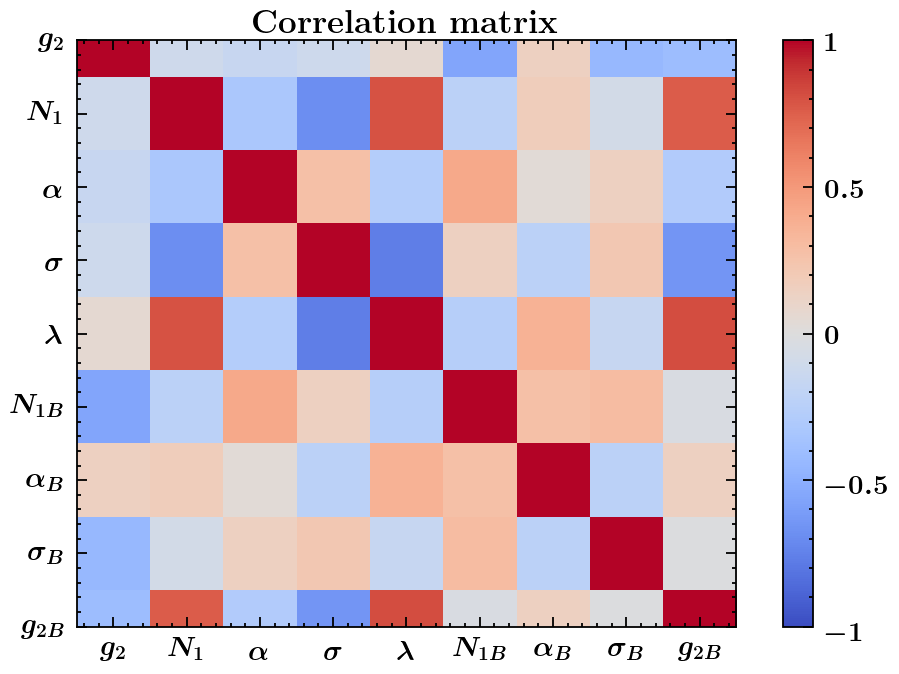
\includegraphics{pngplots/CorrelationMatrix.png}
\caption{Fitted parameter correlation matrix}
\end{figure}

\hypertarget{fit-properties}{%
\subsection{Fit properties}\label{fit-properties}}

\begin{figure}
\centering
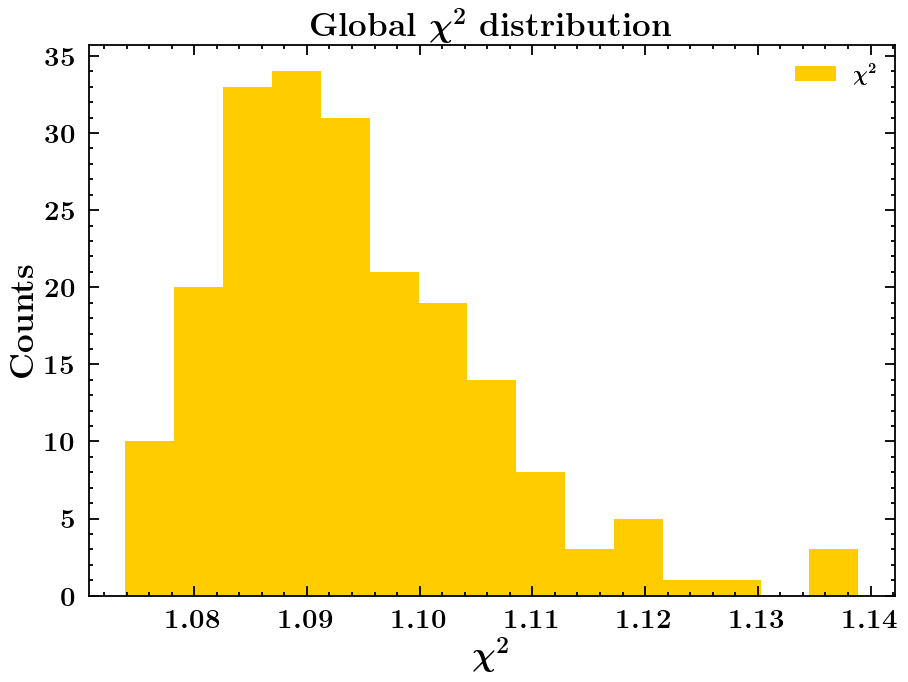
\includegraphics{pngplots/Globalchi2.png}
\caption{Global \(\chi^2\) distribution}
\end{figure}

\begin{figure}
\centering
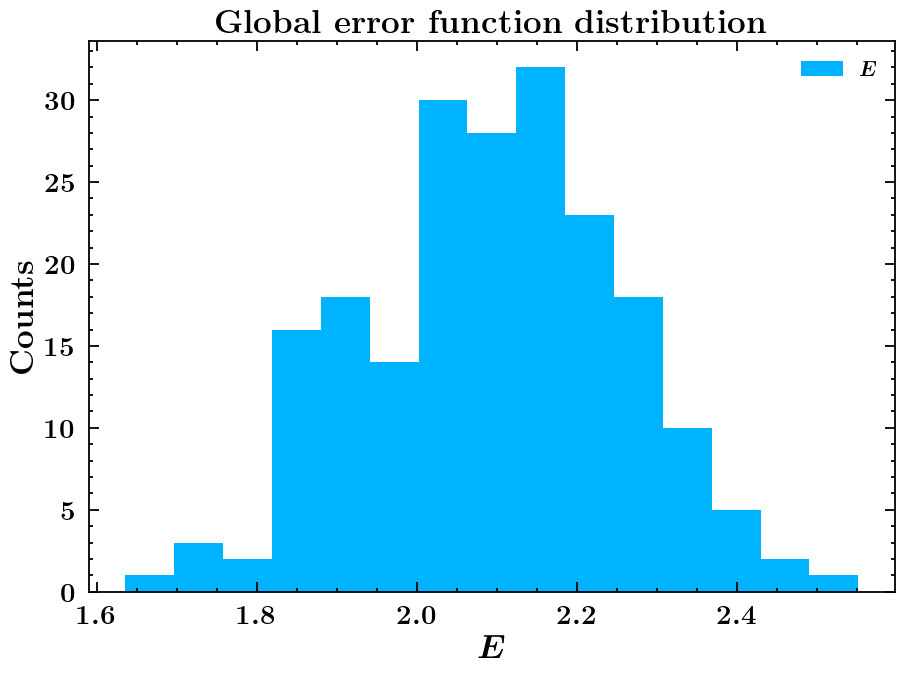
\includegraphics{pngplots/GlobalErrorFunction.png}
\caption{Global error function distribution}
\end{figure}

\begin{figure}
\centering
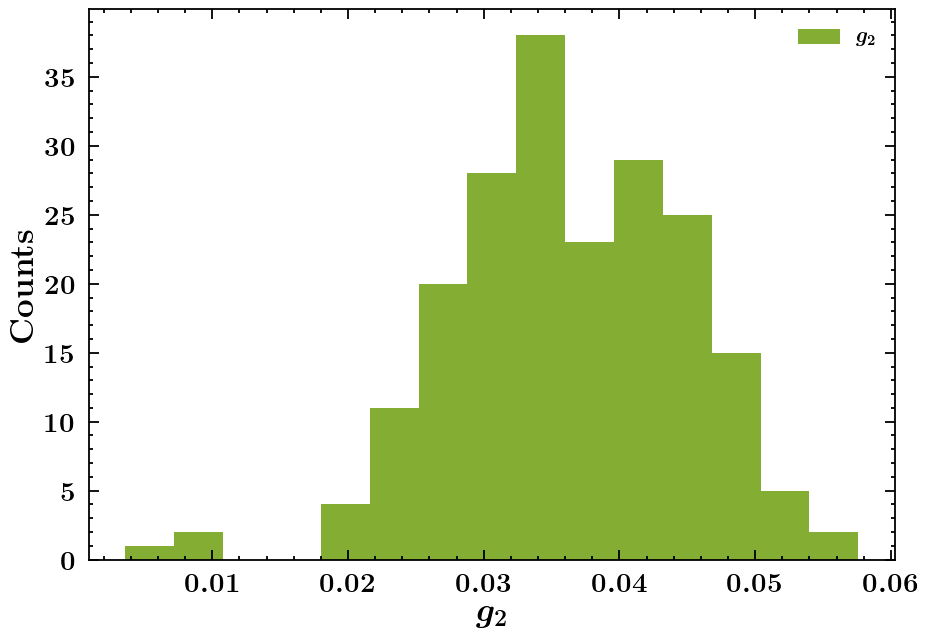
\includegraphics{pngplots/param0.png}
\caption{\(g_2\) distribution}
\end{figure}

\begin{figure}
\centering
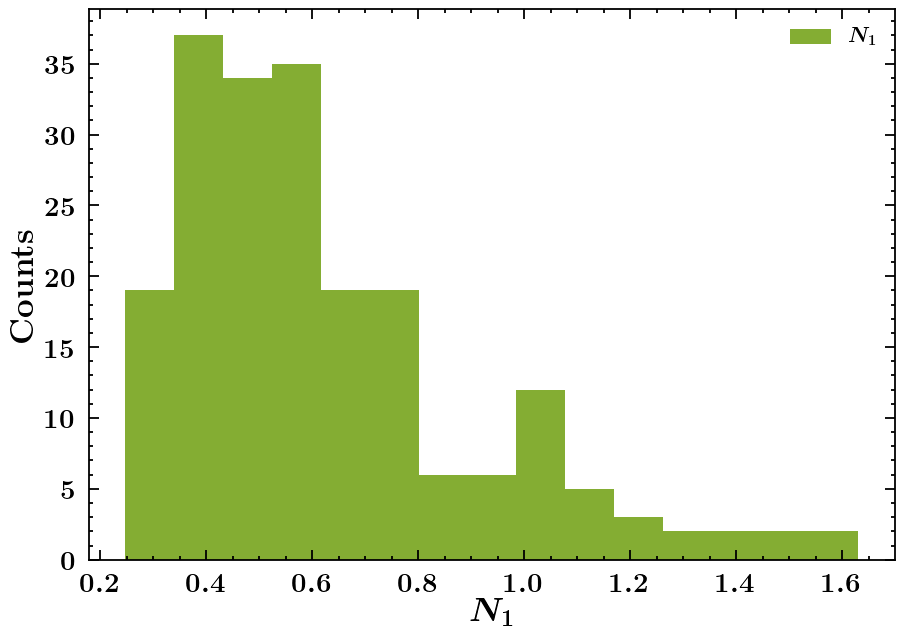
\includegraphics{pngplots/param1.png}
\caption{\(N_1\) distribution}
\end{figure}

\begin{figure}
\centering
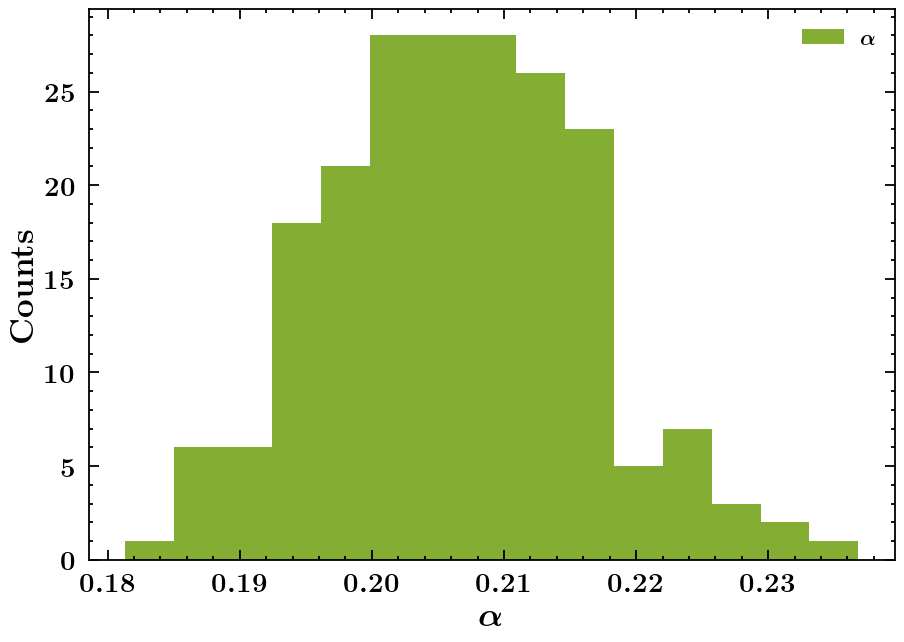
\includegraphics{pngplots/param2.png}
\caption{\(\alpha\) distribution}
\end{figure}

\begin{figure}
\centering
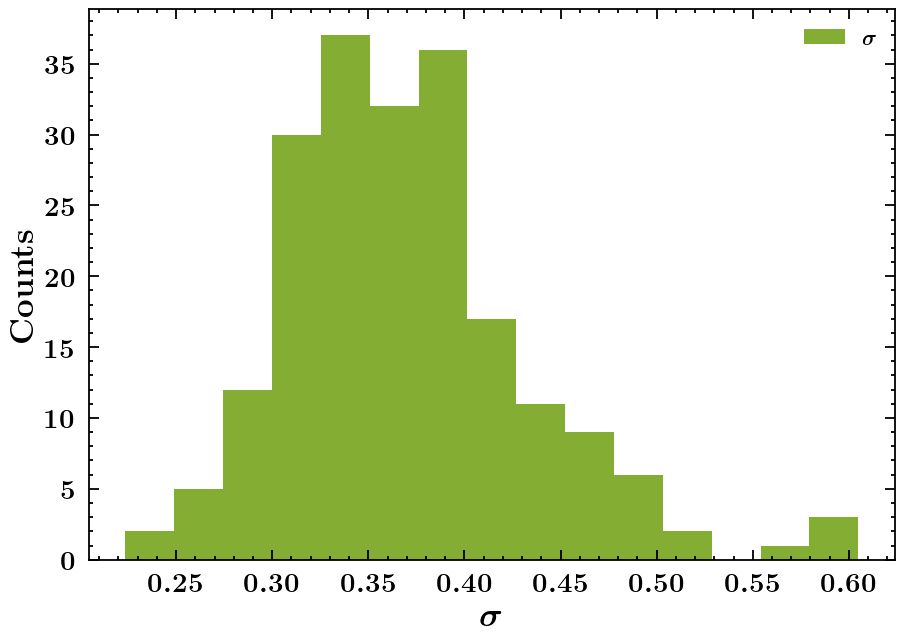
\includegraphics{pngplots/param3.png}
\caption{\(\sigma\) distribution}
\end{figure}

\begin{figure}
\centering
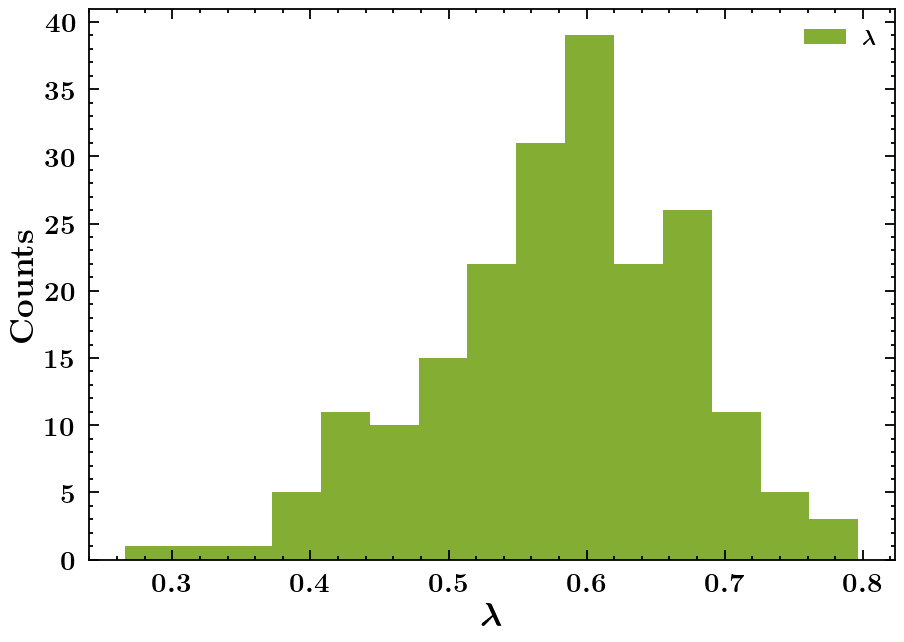
\includegraphics{pngplots/param4.png}
\caption{\(\lambda\) distribution}
\end{figure}

\begin{figure}
\centering
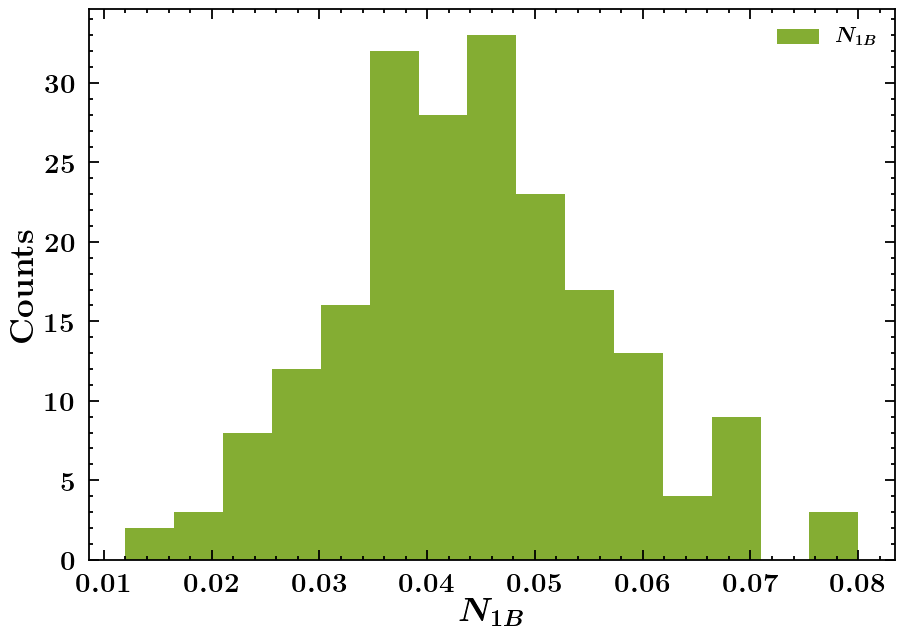
\includegraphics{pngplots/param5.png}
\caption{\(N_{1B}\) distribution}
\end{figure}

\begin{figure}
\centering
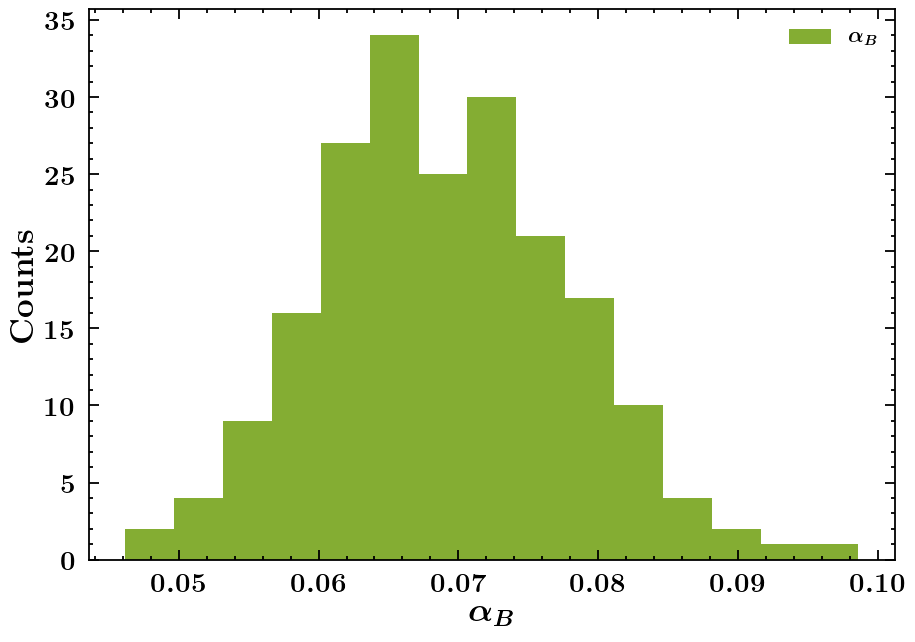
\includegraphics{pngplots/param6.png}
\caption{\(\alpha_B\) distribution}
\end{figure}

\begin{figure}
\centering
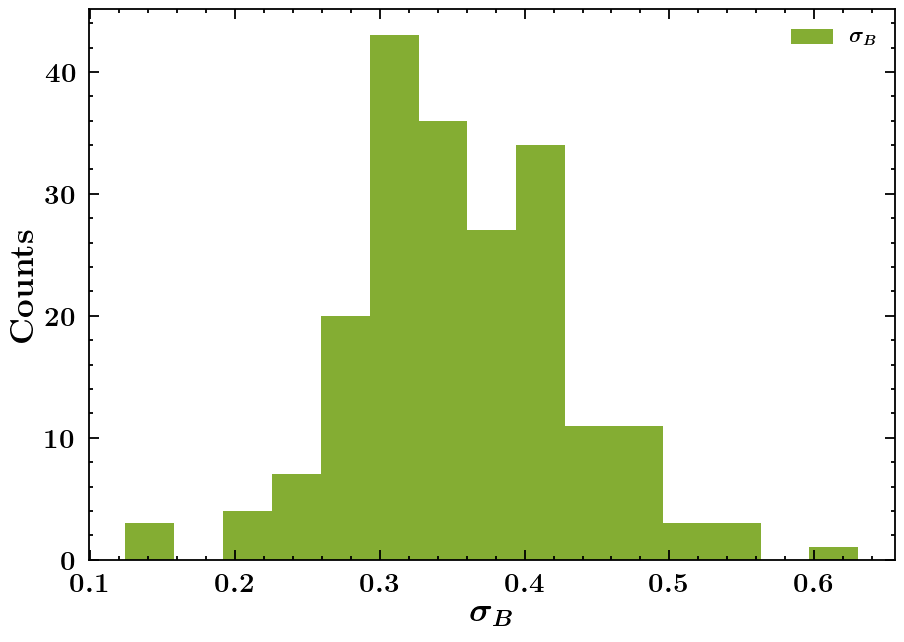
\includegraphics{pngplots/param7.png}
\caption{\(\sigma_B\) distribution}
\end{figure}

\begin{figure}
\centering
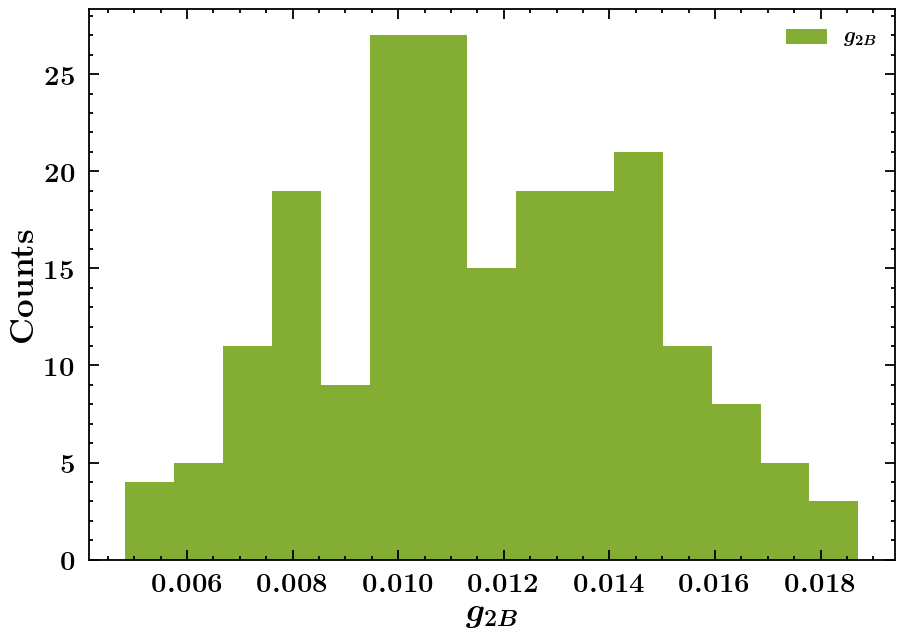
\includegraphics{pngplots/param8.png}
\caption{\(g_{2B}\) distribution}
\end{figure}

\hypertarget{table-of-chi2s}{%
\subsection{\texorpdfstring{Table of
\(\chi^2\)'s}{Table of \textbackslash chi\^{}2's}}\label{table-of-chi2s}}

\begin{table}[h]

\centering

\begin{tabular}{|c|c|c|c|c|} \hline

\textbf{Experiment} & \textbf{Number of
points} & \textbf{\(\chi_{D}^2\)} & \textbf{\(\chi_{\lambda}^2\)} & \textbf{\(\chi^2\)} \\ \hline

E605\_Q\_7\_8 & 7 & 0.67 & 0.01 & 0.68 \\ \hline
E605\_Q\_8\_9 & 8 & 1.52 & 0.0 & 1.52 \\ \hline
E605\_Q\_10.5\_11.5 & 10 & 0.34 & 0.17 & 0.51 \\ \hline
E605\_Q\_11.5\_13.5 & 12 & 0.8 & 0.49 & 1.29 \\ \hline
E605\_Q\_13.5\_18 & 13 & 1.41 & 0.61 & 2.02 \\ \hline
E288\_200\_Q\_4\_5 & 4 & 0.52 & 0.84 & 1.37 \\ \hline
E288\_200\_Q\_5\_6 & 5 & 1.36 & 0.27 & 1.63 \\ \hline
E288\_200\_Q\_6\_7 & 6 & 0.26 & 0.13 & 0.39 \\ \hline
E288\_200\_Q\_7\_8 & 7 & 0.4 & 0.0 & 0.41 \\ \hline
E288\_200\_Q\_8\_9 & 8 & 0.55 & 0.04 & 0.59 \\ \hline
E288\_300\_Q\_4\_5 & 4 & 0.47 & 0.56 & 1.03 \\ \hline
E288\_300\_Q\_5\_6 & 5 & 0.76 & 0.16 & 0.91 \\ \hline
E288\_300\_Q\_6\_7 & 6 & 0.41 & 0.03 & 0.45 \\ \hline
E288\_300\_Q\_7\_8 & 7 & 0.09 & 0.01 & 0.1 \\ \hline
E288\_300\_Q\_8\_9 & 8 & 0.55 & 0.0 & 0.56 \\ \hline
E288\_300\_Q\_11\_12 & 9 & 0.36 & 0.25 & 0.61 \\ \hline
E288\_400\_Q\_5\_6 & 5 & 0.27 & 0.01 & 0.28 \\ \hline
E288\_400\_Q\_6\_7 & 6 & 0.08 & 0.0 & 0.08 \\ \hline
E288\_400\_Q\_7\_8 & 7 & 0.02 & 0.02 & 0.04 \\ \hline
E288\_400\_Q\_8\_9 & 8 & 0.41 & 0.05 & 0.46 \\ \hline
E288\_400\_Q\_11\_12 & 11 & 0.51 & 0.05 & 0.56 \\ \hline
E288\_400\_Q\_12\_13 & 12 & 0.49 & 0.05 & 0.54 \\ \hline
E288\_400\_Q\_13\_14 & 12 & 0.59 & 0.09 & 0.68 \\ \hline
STAR\_510 & 7 & 0.89 & 0.03 & 0.92 \\ \hline
CDF\_RunI & 25 & 0.53 & 0.06 & 0.59 \\ \hline
CDF\_RunII & 26 & 0.87 & 0.0 & 0.88 \\ \hline
D0\_RunI & 12 & 0.63 & 0.05 & 0.67 \\ \hline
D0\_RunII & 5 & 1.13 & 0.61 & 1.74 \\ \hline
D0\_RunIImu & 3 & 3.28 & 0.03 & 3.31 \\ \hline
LHCb\_7TeV & 7 & 1.13 & 0.16 & 1.28 \\ \hline
LHCb\_8TeV & 7 & 0.54 & 0.08 & 0.62 \\ \hline
LHCb\_13TeV & 7 & 0.79 & 0.02 & 0.81 \\ \hline
CMS\_7TeV & 4 & 2.13 & 0 & 2.13 \\ \hline
CMS\_8TeV & 4 & 1.43 & 0.01 & 1.43 \\ \hline
ATLAS\_7TeV\_y\_0\_1 & 6 & 2.65 & 0.03 & 2.68 \\ \hline
ATLAS\_7TeV\_y\_1\_2 & 6 & 4.2 & 1.03 & 5.24 \\ \hline
ATLAS\_7TeV\_y\_2\_2.4 & 6 & 3.51 & 0.38 & 3.9 \\ \hline
ATLAS\_8TeV\_y\_0\_0.4 & 6 & 2.0 & 0.35 & 2.36 \\ \hline
ATLAS\_8TeV\_y\_0.4\_0.8 & 6 & 2.2 & 0.27 & 2.47 \\ \hline
ATLAS\_8TeV\_y\_0.8\_1.2 & 6 & 0.89 & 0.06 & 0.96 \\ \hline
ATLAS\_8TeV\_y\_1.2\_1.6 & 6 & 0.91 & 0.1 & 1.02 \\ \hline
ATLAS\_8TeV\_y\_1.6\_2 & 6 & 0.61 & 0.08 & 0.69 \\ \hline
ATLAS\_8TeV\_y\_2\_2.4 & 6 & 0.72 & 0.3 & 1.02 \\ \hline
ATLAS\_8TeV\_Q\_46\_66 & 4 & 2.3 & 0.7 & 3.0 \\ \hline
ATLAS\_8TeV\_Q\_116\_150 & 8 & 0.5 & 0.0 & 0.5 \\ \hline
Total & 353 & - & - & 1.07 \\ \hline

\end{tabular}

\caption{Central-replica \(\chi^2\)'s:}

\end{table}

\begin{table}[h]

\centering

\begin{tabular}{|c|c|c|c|c|} \hline

\textbf{Experiment} & \textbf{Number of
points} & \textbf{\(\chi_{D}^2\)} & \textbf{\(\chi_{\lambda}^2\)} & \textbf{\(\chi^2\)} \\ \hline

E605\_Q\_7\_8 & 7 & 0.42 & 0.07 & 0.49 \\ \hline
E605\_Q\_8\_9 & 8 & 0.99 & 0.03 & 1.03 \\ \hline
E605\_Q\_10.5\_11.5 & 10 & 0.19 & 0.14 & 0.33 \\ \hline
E605\_Q\_11.5\_13.5 & 12 & 0.49 & 0.28 & 0.77 \\ \hline
E605\_Q\_13.5\_18 & 13 & 0.49 & 0.39 & 0.88 \\ \hline
E288\_200\_Q\_4\_5 & 4 & 0.21 & 0.65 & 0.86 \\ \hline
E288\_200\_Q\_5\_6 & 5 & 0.67 & 0.29 & 0.96 \\ \hline
E288\_200\_Q\_6\_7 & 6 & 0.13 & 0.14 & 0.27 \\ \hline
E288\_200\_Q\_7\_8 & 7 & 0.25 & 0.01 & 0.27 \\ \hline
E288\_200\_Q\_8\_9 & 8 & 0.65 & 0.02 & 0.68 \\ \hline
E288\_300\_Q\_4\_5 & 4 & 0.23 & 0.55 & 0.79 \\ \hline
E288\_300\_Q\_5\_6 & 5 & 0.5 & 0.2 & 0.71 \\ \hline
E288\_300\_Q\_6\_7 & 6 & 0.32 & 0.06 & 0.38 \\ \hline
E288\_300\_Q\_7\_8 & 7 & 0.06 & 0.03 & 0.09 \\ \hline
E288\_300\_Q\_8\_9 & 8 & 0.53 & 0.02 & 0.55 \\ \hline
E288\_300\_Q\_11\_12 & 9 & 1.05 & 0.17 & 1.21 \\ \hline
E288\_400\_Q\_5\_6 & 5 & 0.31 & 0.07 & 0.38 \\ \hline
E288\_400\_Q\_6\_7 & 6 & 0.1 & 0.0 & 0.1 \\ \hline
E288\_400\_Q\_7\_8 & 7 & 0.02 & 0.01 & 0.03 \\ \hline
E288\_400\_Q\_8\_9 & 8 & 0.44 & 0.04 & 0.48 \\ \hline
E288\_400\_Q\_11\_12 & 11 & 0.64 & 0.04 & 0.67 \\ \hline
E288\_400\_Q\_12\_13 & 12 & 0.79 & 0.03 & 0.82 \\ \hline
E288\_400\_Q\_13\_14 & 12 & 1.06 & 0.04 & 1.11 \\ \hline
STAR\_510 & 7 & 0.78 & 0.05 & 0.84 \\ \hline
CDF\_RunI & 25 & 0.48 & 0.06 & 0.54 \\ \hline
CDF\_RunII & 26 & 0.96 & 0.0 & 0.96 \\ \hline
D0\_RunI & 12 & 0.71 & 0.04 & 0.75 \\ \hline
D0\_RunII & 5 & 1.33 & 0.61 & 1.94 \\ \hline
D0\_RunIImu & 3 & 3.2 & 0.02 & 3.22 \\ \hline
LHCb\_7TeV & 7 & 1.07 & 0.19 & 1.26 \\ \hline
LHCb\_8TeV & 7 & 0.46 & 0.07 & 0.53 \\ \hline
LHCb\_13TeV & 7 & 0.74 & 0.02 & 0.75 \\ \hline
CMS\_7TeV & 4 & 2.13 & 0 & 2.13 \\ \hline
CMS\_8TeV & 4 & 1.41 & 0.01 & 1.41 \\ \hline
ATLAS\_7TeV\_y\_0\_1 & 6 & 2.58 & 0.03 & 2.61 \\ \hline
ATLAS\_7TeV\_y\_1\_2 & 6 & 4.33 & 1.03 & 5.36 \\ \hline
ATLAS\_7TeV\_y\_2\_2.4 & 6 & 3.56 & 0.38 & 3.94 \\ \hline
ATLAS\_8TeV\_y\_0\_0.4 & 6 & 1.92 & 0.34 & 2.26 \\ \hline
ATLAS\_8TeV\_y\_0.4\_0.8 & 6 & 2.34 & 0.25 & 2.59 \\ \hline
ATLAS\_8TeV\_y\_0.8\_1.2 & 6 & 0.92 & 0.06 & 0.98 \\ \hline
ATLAS\_8TeV\_y\_1.2\_1.6 & 6 & 0.91 & 0.09 & 1.01 \\ \hline
ATLAS\_8TeV\_y\_1.6\_2 & 6 & 0.72 & 0.09 & 0.81 \\ \hline
ATLAS\_8TeV\_y\_2\_2.4 & 6 & 0.93 & 0.35 & 1.28 \\ \hline
ATLAS\_8TeV\_Q\_46\_66 & 4 & 2.14 & 0.74 & 2.88 \\ \hline
ATLAS\_8TeV\_Q\_116\_150 & 8 & 0.5 & 0.0 & 0.5 \\ \hline
Total & 353 & - & - & 1.02 \\ \hline

\end{tabular}

\caption{Mean-replica \(\chi^2\)'s:}

\end{table}

\begin{table}[h]

\centering

\begin{tabular}{|c|c|c|} \hline

\textbf{Experiment} & \textbf{Number of
points} & \textbf{\(\chi^2\)} \\ \hline

E605\_Q\_7\_8 & 7 & 0.69 \(\pm\) 0.11 \\ \hline
E605\_Q\_8\_9 & 8 & 1.54 \(\pm\) 0.22 \\ \hline
E605\_Q\_10.5\_11.5 & 10 & 0.55 \(\pm\) 0.07 \\ \hline
E605\_Q\_11.5\_13.5 & 12 & 1.39 \(\pm\) 0.11 \\ \hline
E605\_Q\_13.5\_18 & 13 & 2.04 \(\pm\) 0.11 \\ \hline
E288\_200\_Q\_4\_5 & 4 & 1.43 \(\pm\) 0.29 \\ \hline
E288\_200\_Q\_5\_6 & 5 & 1.67 \(\pm\) 0.2 \\ \hline
E288\_200\_Q\_6\_7 & 6 & 0.42 \(\pm\) 0.08 \\ \hline
E288\_200\_Q\_7\_8 & 7 & 0.43 \(\pm\) 0.14 \\ \hline
E288\_200\_Q\_8\_9 & 8 & 0.6 \(\pm\) 0.07 \\ \hline
E288\_300\_Q\_4\_5 & 4 & 1.09 \(\pm\) 0.27 \\ \hline
E288\_300\_Q\_5\_6 & 5 & 0.94 \(\pm\) 0.14 \\ \hline
E288\_300\_Q\_6\_7 & 6 & 0.46 \(\pm\) 0.13 \\ \hline
E288\_300\_Q\_7\_8 & 7 & 0.12 \(\pm\) 0.04 \\ \hline
E288\_300\_Q\_8\_9 & 8 & 0.58 \(\pm\) 0.1 \\ \hline
E288\_300\_Q\_11\_12 & 9 & 0.61 \(\pm\) 0.03 \\ \hline
E288\_400\_Q\_5\_6 & 5 & 0.32 \(\pm\) 0.08 \\ \hline
E288\_400\_Q\_6\_7 & 6 & 0.11 \(\pm\) 0.03 \\ \hline
E288\_400\_Q\_7\_8 & 7 & 0.08 \(\pm\) 0.05 \\ \hline
E288\_400\_Q\_8\_9 & 8 & 0.5 \(\pm\) 0.08 \\ \hline
E288\_400\_Q\_11\_12 & 11 & 0.6 \(\pm\) 0.14 \\ \hline
E288\_400\_Q\_12\_13 & 12 & 0.57 \(\pm\) 0.04 \\ \hline
E288\_400\_Q\_13\_14 & 12 & 0.7 \(\pm\) 0.05 \\ \hline
STAR\_510 & 7 & 0.93 \(\pm\) 0.05 \\ \hline
CDF\_RunI & 25 & 0.59 \(\pm\) 0.02 \\ \hline
CDF\_RunII & 26 & 0.9 \(\pm\) 0.07 \\ \hline
D0\_RunI & 12 & 0.67 \(\pm\) 0.03 \\ \hline
D0\_RunII & 5 & 1.7 \(\pm\) 0.22 \\ \hline
D0\_RunIImu & 3 & 3.21 \(\pm\) 0.44 \\ \hline
LHCb\_7TeV & 7 & 1.28 \(\pm\) 0.04 \\ \hline
LHCb\_8TeV & 7 & 0.67 \(\pm\) 0.13 \\ \hline
LHCb\_13TeV & 7 & 0.85 \(\pm\) 0.07 \\ \hline
CMS\_7TeV & 4 & 2.13 \(\pm\) 0.01 \\ \hline
CMS\_8TeV & 4 & 1.43 \(\pm\) 0.05 \\ \hline
ATLAS\_7TeV\_y\_0\_1 & 6 & 2.71 \(\pm\) 0.24 \\ \hline
ATLAS\_7TeV\_y\_1\_2 & 6 & 5.29 \(\pm\) 0.09 \\ \hline
ATLAS\_7TeV\_y\_2\_2.4 & 6 & 3.92 \(\pm\) 0.11 \\ \hline
ATLAS\_8TeV\_y\_0\_0.4 & 6 & 2.36 \(\pm\) 0.13 \\ \hline
ATLAS\_8TeV\_y\_0.4\_0.8 & 6 & 2.5 \(\pm\) 0.09 \\ \hline
ATLAS\_8TeV\_y\_0.8\_1.2 & 6 & 0.99 \(\pm\) 0.08 \\ \hline
ATLAS\_8TeV\_y\_1.2\_1.6 & 6 & 1.04 \(\pm\) 0.15 \\ \hline
ATLAS\_8TeV\_y\_1.6\_2 & 6 & 0.8 \(\pm\) 0.24 \\ \hline
ATLAS\_8TeV\_y\_2\_2.4 & 6 & 1.05 \(\pm\) 0.22 \\ \hline
ATLAS\_8TeV\_Q\_46\_66 & 4 & 2.99 \(\pm\) 0.12 \\ \hline
ATLAS\_8TeV\_Q\_116\_150 & 8 & 0.5 \(\pm\) 0.01 \\ \hline
Total & 353 & 1.09 \(\pm\) 0.01 \\ \hline

\end{tabular}

\caption{Average-over-replicas \(\chi^2\)'s:}

\end{table}

\hypertarget{tmds-in-k_t-space}{%
\subsection{\texorpdfstring{TMDs in \(k_T\)
space}{TMDs in k\_T space}}\label{tmds-in-k_t-space}}

\begin{figure}
\centering
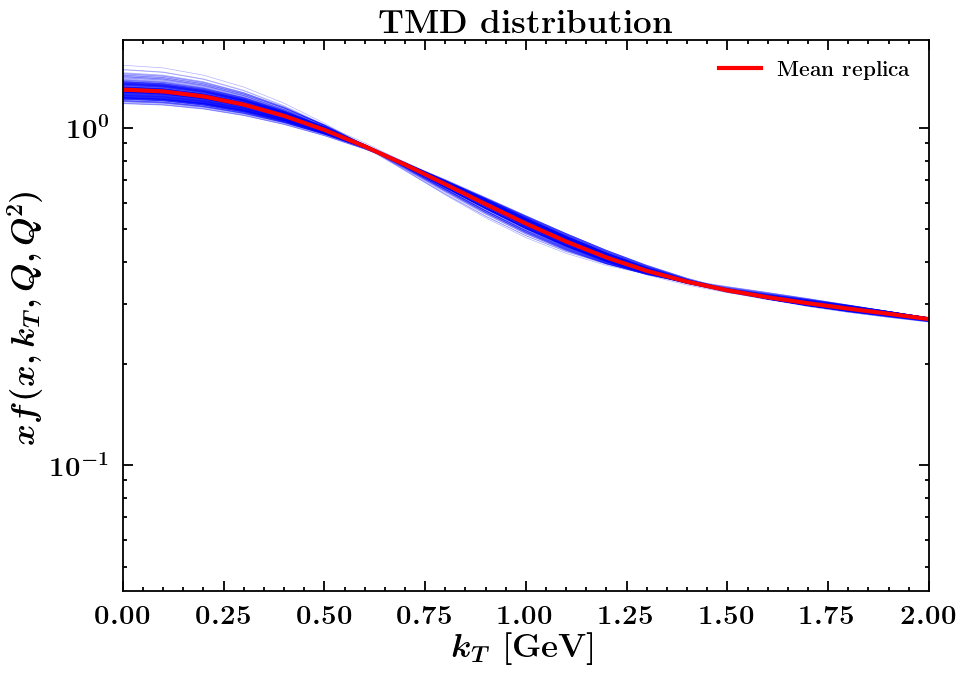
\includegraphics{pngplots/tmd_1_2_0.001.png}
\caption{TMD PDF of the \(d\) at \(Q = 2\) GeV and \(x = 0.001\)}
\end{figure}

\begin{figure}
\centering
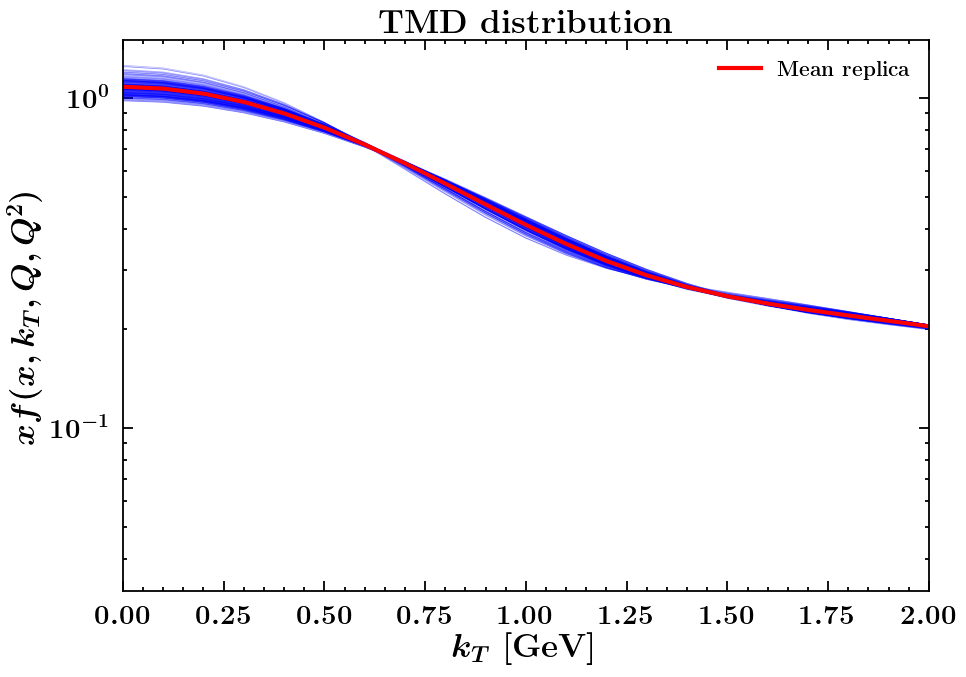
\includegraphics{pngplots/tmd_1_2_0.01.png}
\caption{TMD PDF of the \(d\) at \(Q = 2\) GeV and \(x = 0.01\)}
\end{figure}

\begin{figure}
\centering
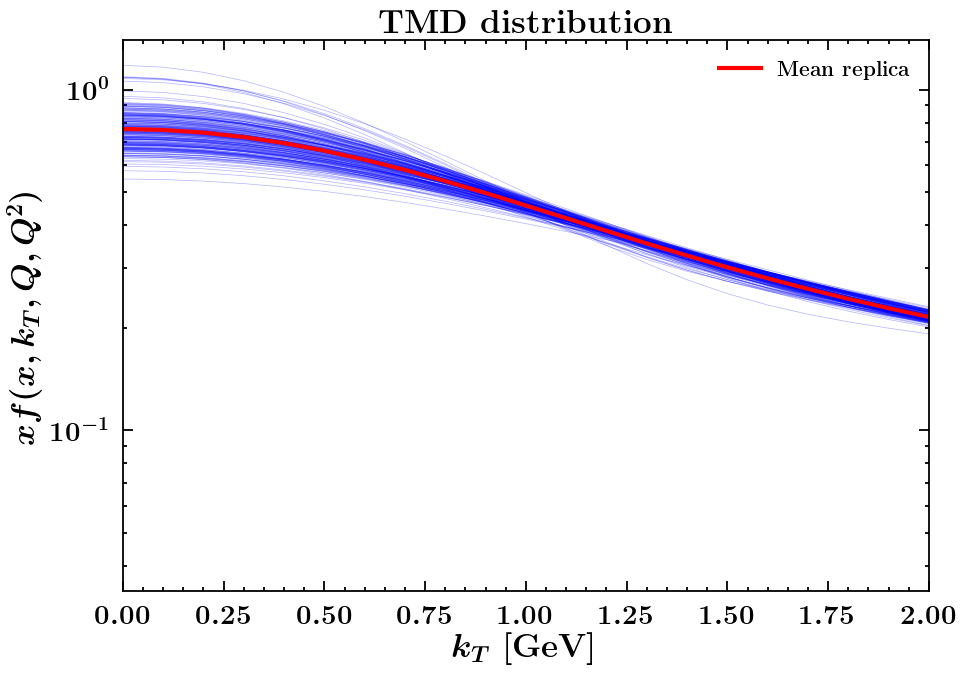
\includegraphics{pngplots/tmd_1_2_0.1.png}
\caption{TMD PDF of the \(d\) at \(Q = 2\) GeV and \(x = 0.1\)}
\end{figure}

\begin{figure}
\centering
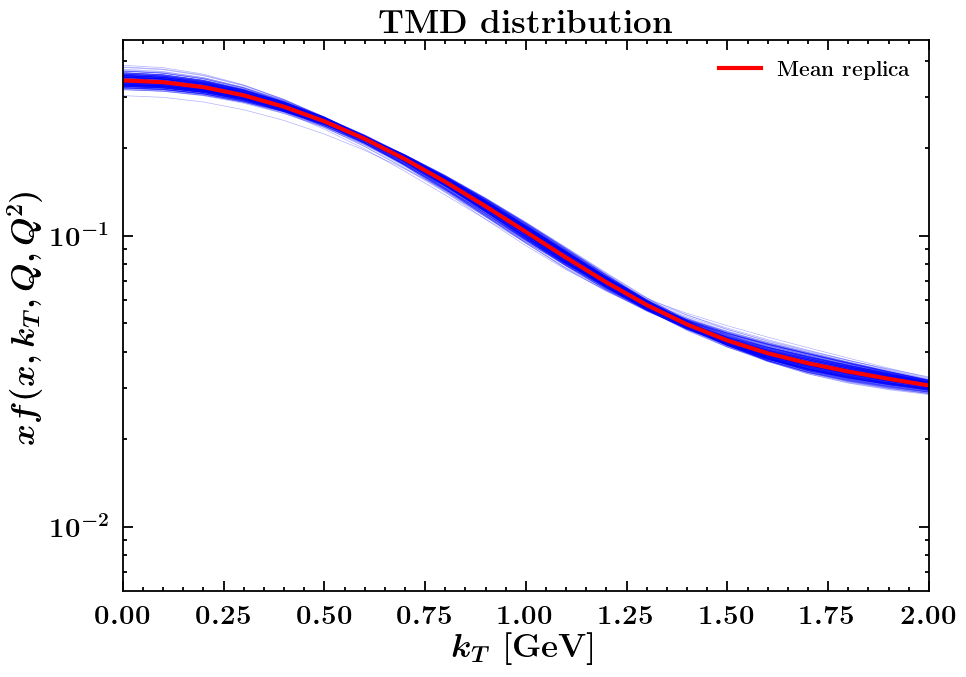
\includegraphics{pngplots/tmd_1_2_0.5.png}
\caption{TMD PDF of the \(d\) at \(Q = 2\) GeV and \(x = 0.5\)}
\end{figure}

\begin{figure}
\centering
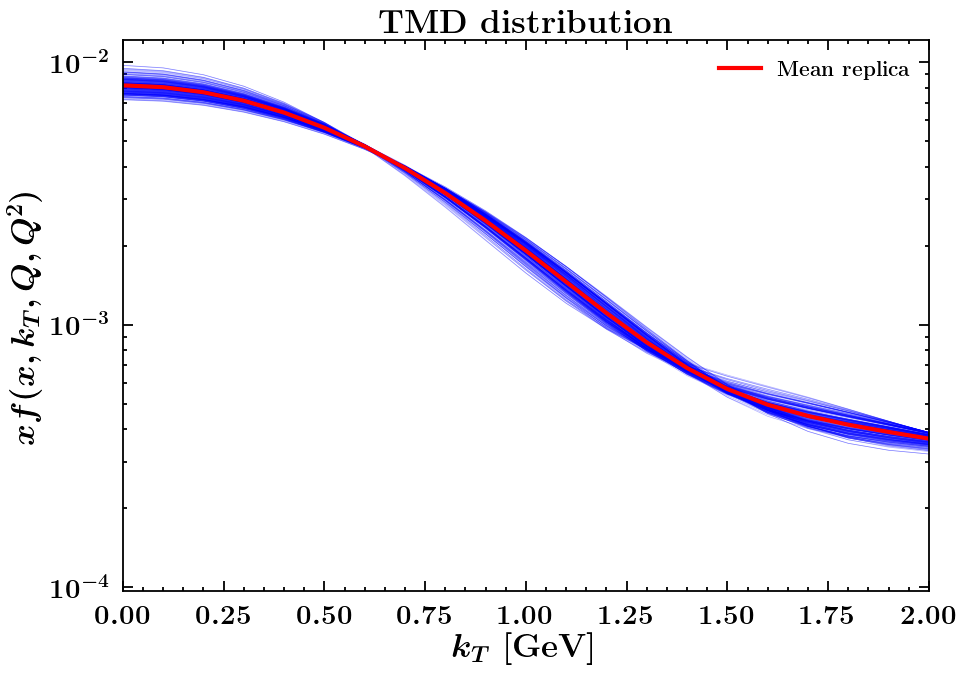
\includegraphics{pngplots/tmd_1_2_0.9.png}
\caption{TMD PDF of the \(d\) at \(Q = 2\) GeV and \(x = 0.9\)}
\end{figure}

\hypertarget{data-theory-comparison}{%
\subsection{Data-theory comparison}\label{data-theory-comparison}}

\begin{figure}
\centering
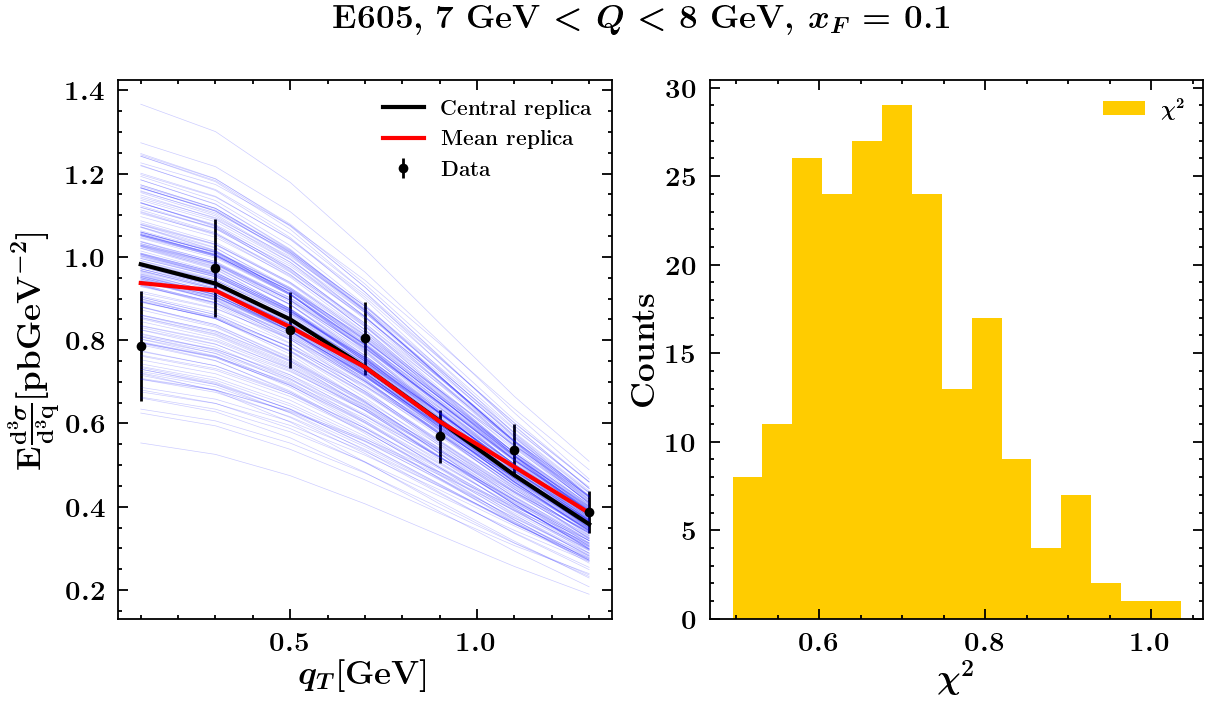
\includegraphics{pngplots/E605_Q_7_8.png}
\caption{E605\_Q\_7\_8 data-theory comparison}
\end{figure}

\begin{figure}
\centering
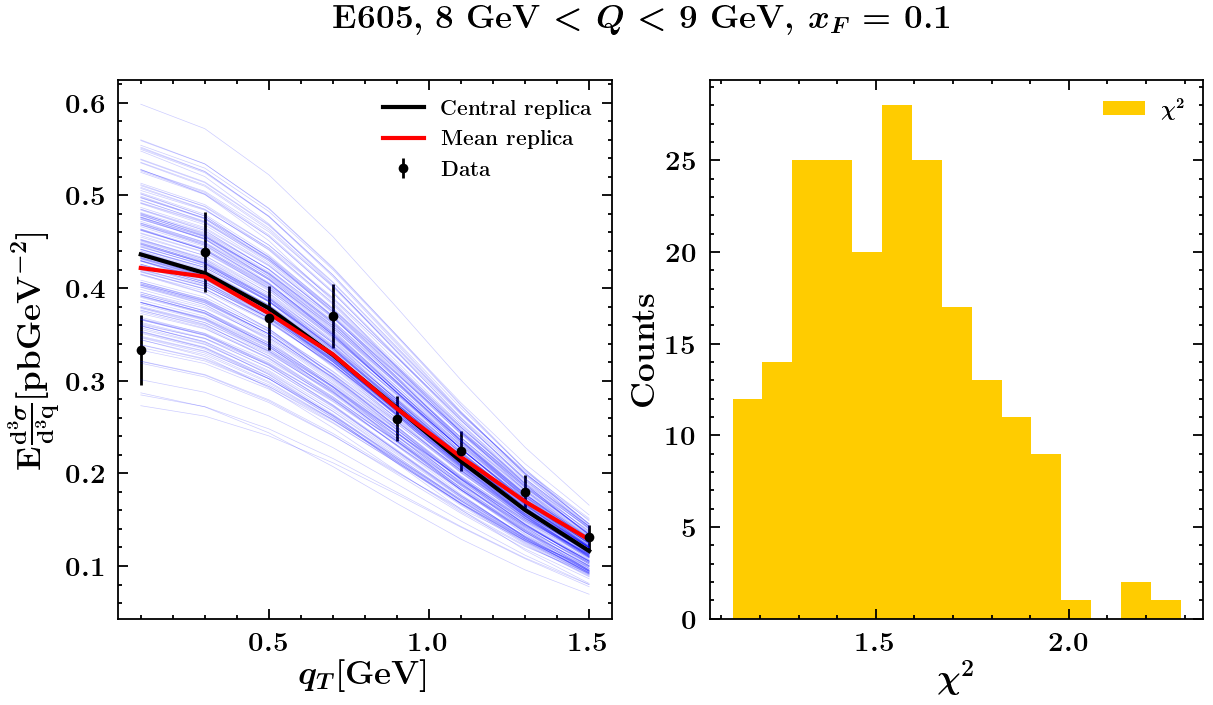
\includegraphics{pngplots/E605_Q_8_9.png}
\caption{E605\_Q\_8\_9 data-theory comparison}
\end{figure}

\begin{figure}
\centering
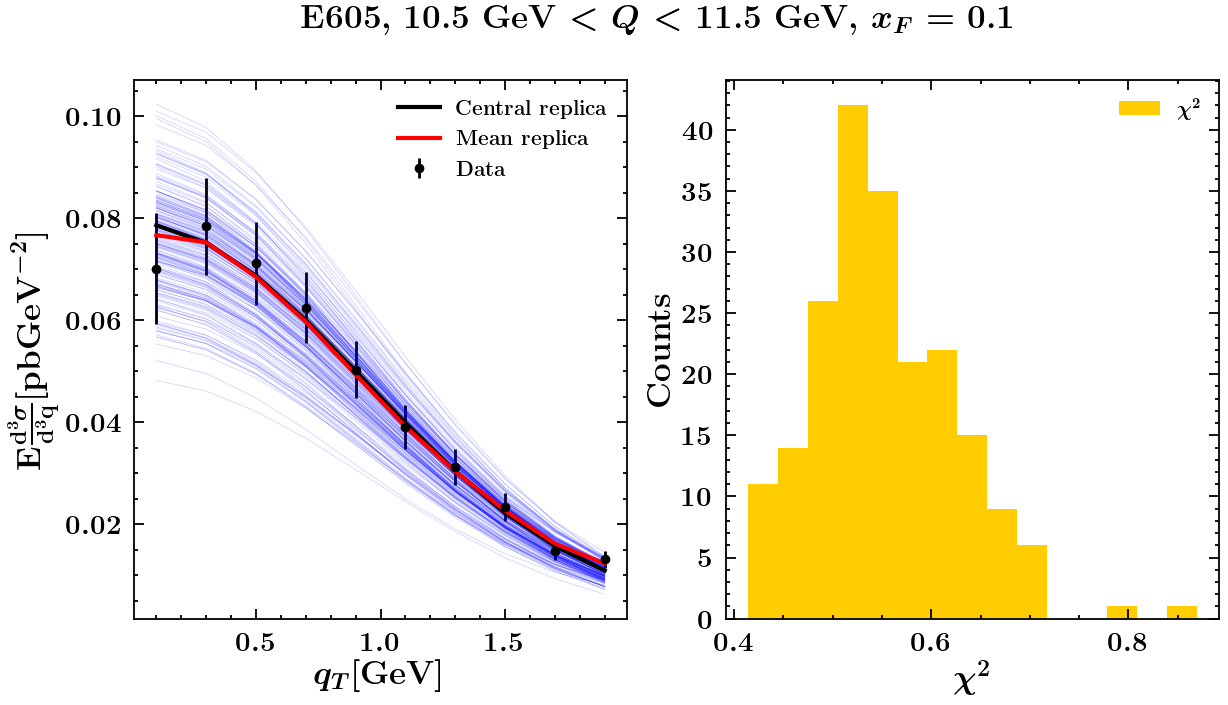
\includegraphics{pngplots/E605_Q_10.5_11.5.png}
\caption{E605\_Q\_10.5\_11.5 data-theory comparison}
\end{figure}

\begin{figure}
\centering
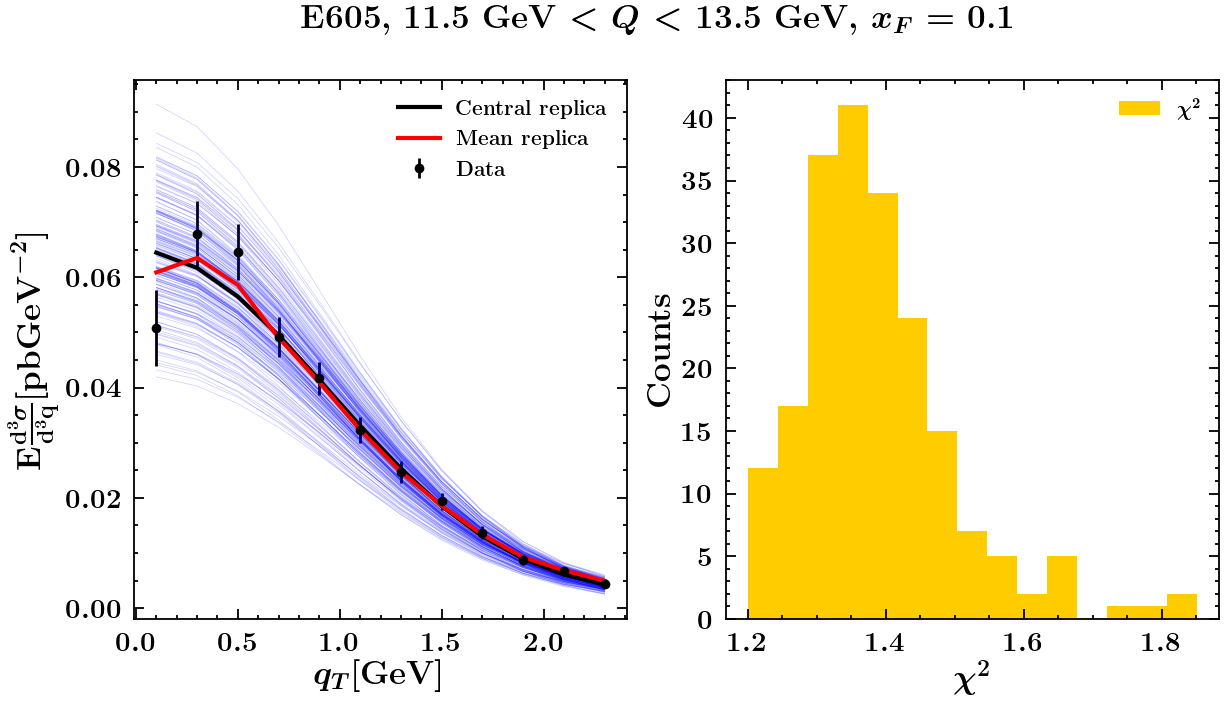
\includegraphics{pngplots/E605_Q_11.5_13.5.png}
\caption{E605\_Q\_11.5\_13.5 data-theory comparison}
\end{figure}

\begin{figure}
\centering
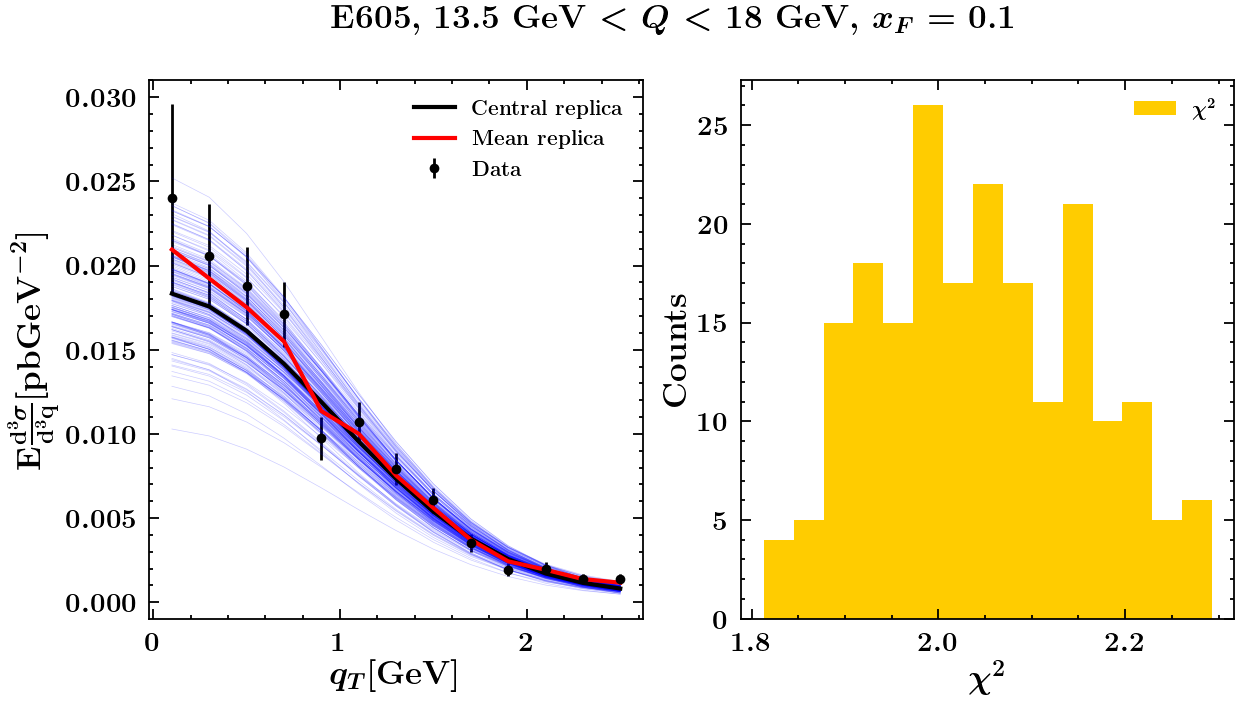
\includegraphics{pngplots/E605_Q_13.5_18.png}
\caption{E605\_Q\_13.5\_18 data-theory comparison}
\end{figure}

\begin{figure}
\centering
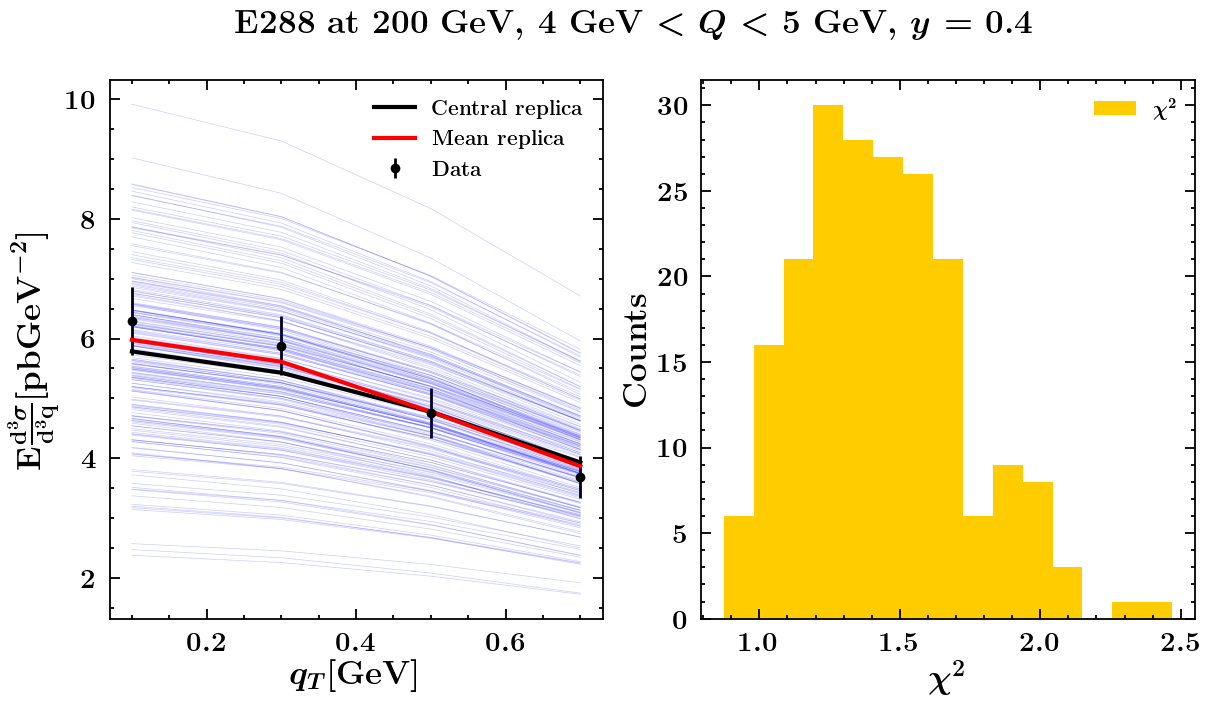
\includegraphics{pngplots/E288_200_Q_4_5.png}
\caption{E288\_200\_Q\_4\_5 data-theory comparison}
\end{figure}

\begin{figure}
\centering
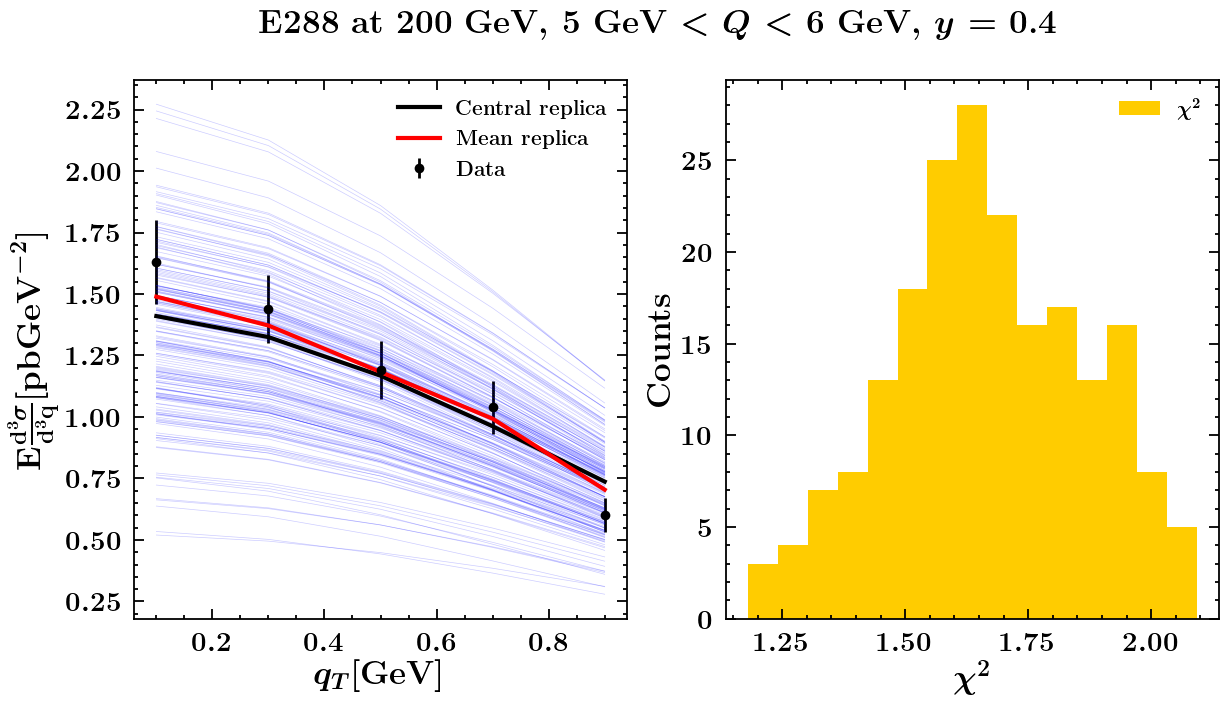
\includegraphics{pngplots/E288_200_Q_5_6.png}
\caption{E288\_200\_Q\_5\_6 data-theory comparison}
\end{figure}

\begin{figure}
\centering
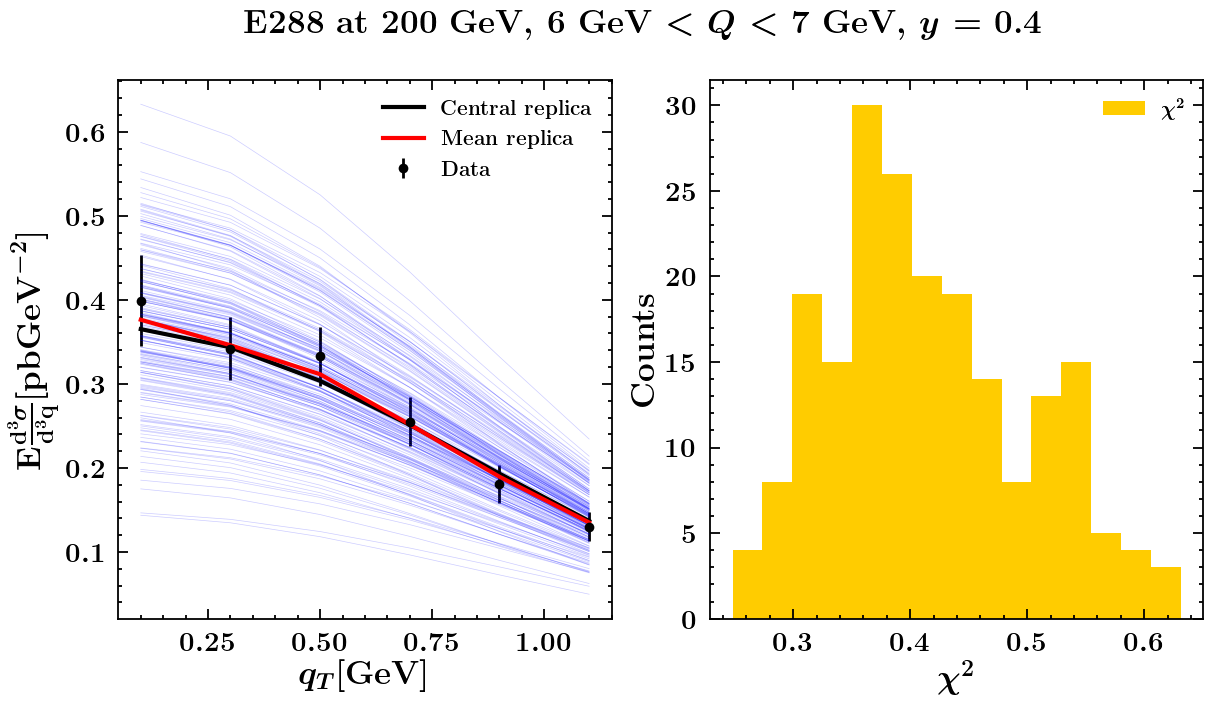
\includegraphics{pngplots/E288_200_Q_6_7.png}
\caption{E288\_200\_Q\_6\_7 data-theory comparison}
\end{figure}

\begin{figure}
\centering
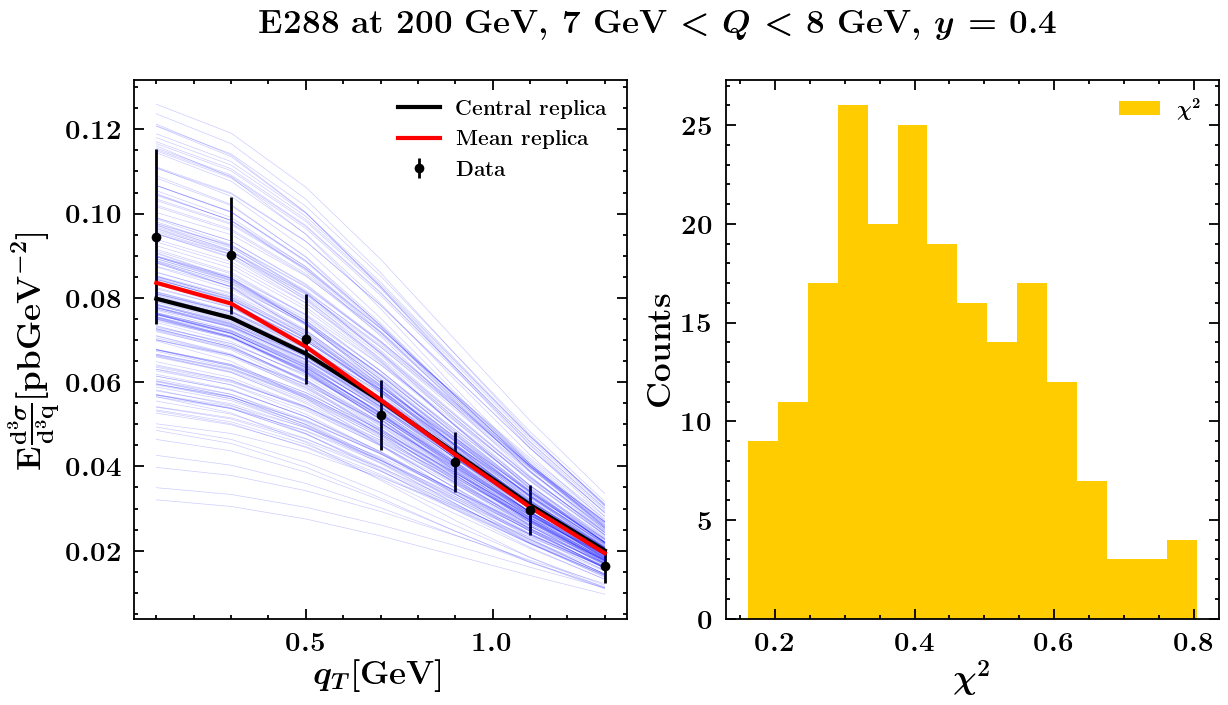
\includegraphics{pngplots/E288_200_Q_7_8.png}
\caption{E288\_200\_Q\_7\_8 data-theory comparison}
\end{figure}

\begin{figure}
\centering
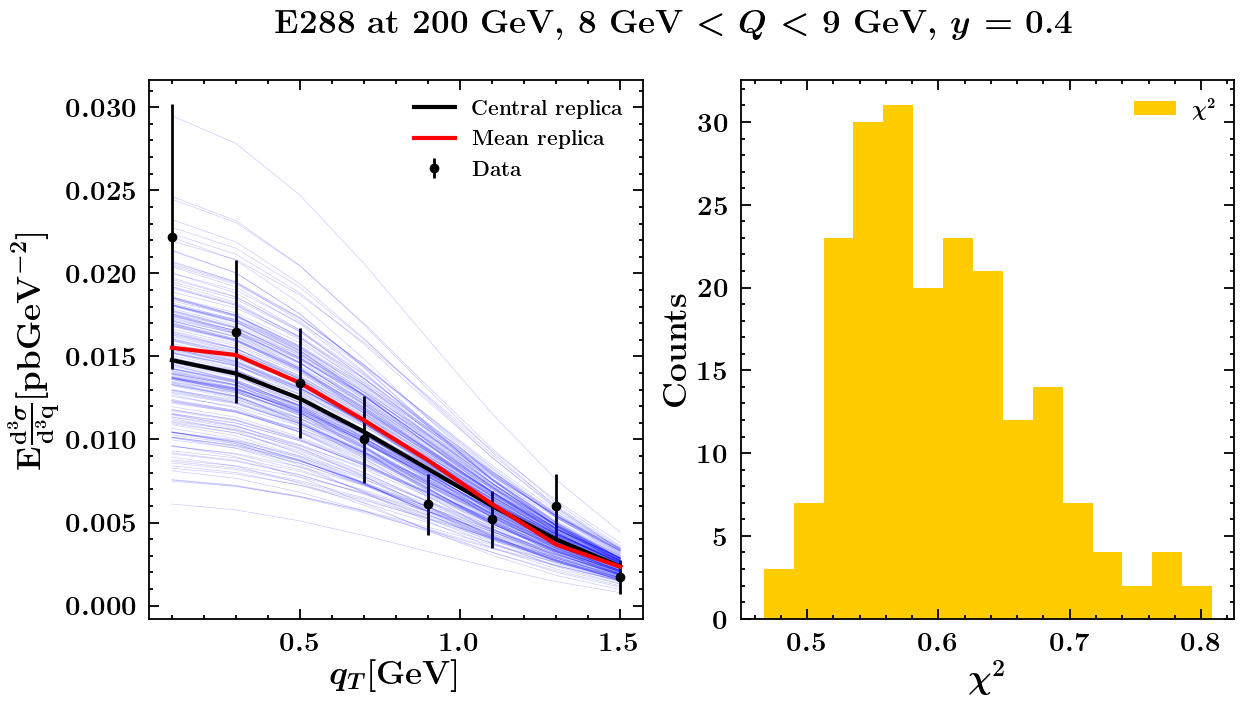
\includegraphics{pngplots/E288_200_Q_8_9.png}
\caption{E288\_200\_Q\_8\_9 data-theory comparison}
\end{figure}

\begin{figure}
\centering
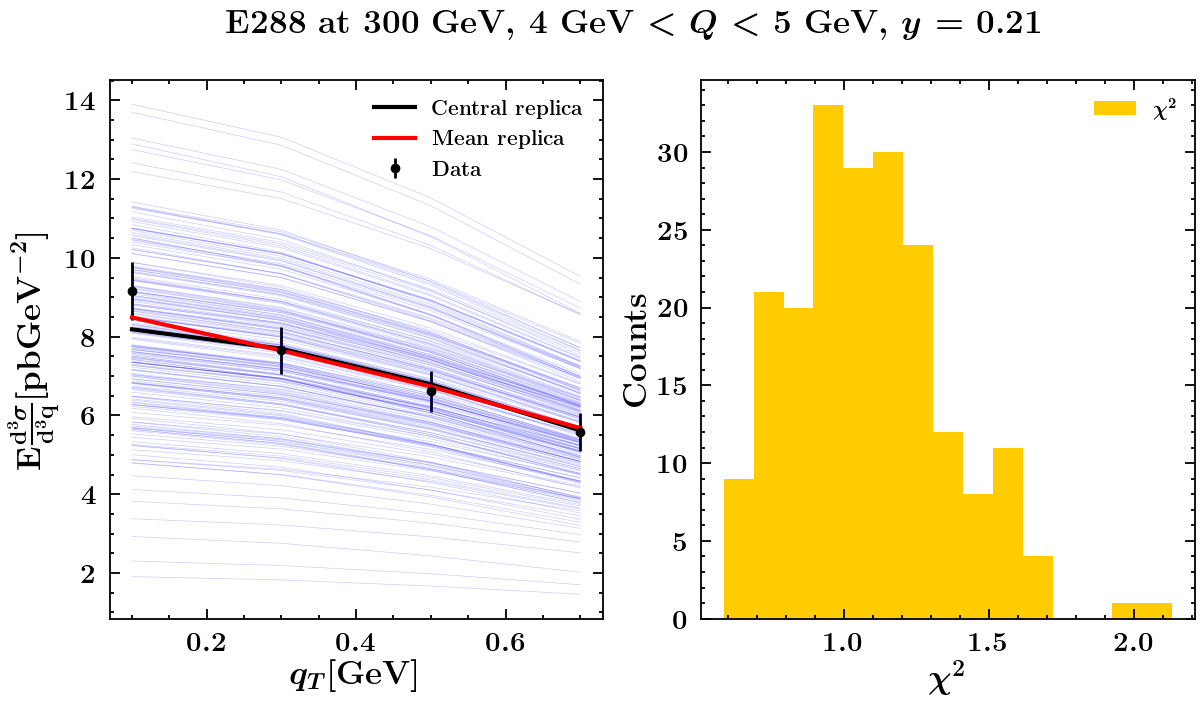
\includegraphics{pngplots/E288_300_Q_4_5.png}
\caption{E288\_300\_Q\_4\_5 data-theory comparison}
\end{figure}

\begin{figure}
\centering
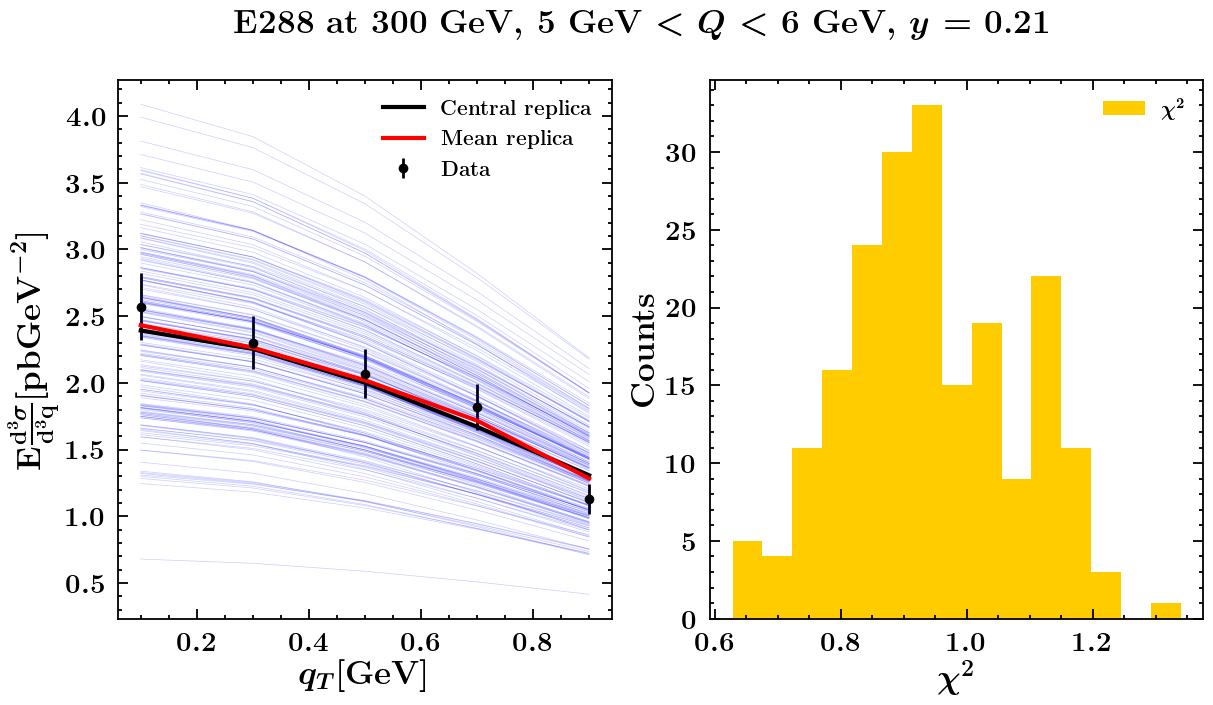
\includegraphics{pngplots/E288_300_Q_5_6.png}
\caption{E288\_300\_Q\_5\_6 data-theory comparison}
\end{figure}

\begin{figure}
\centering
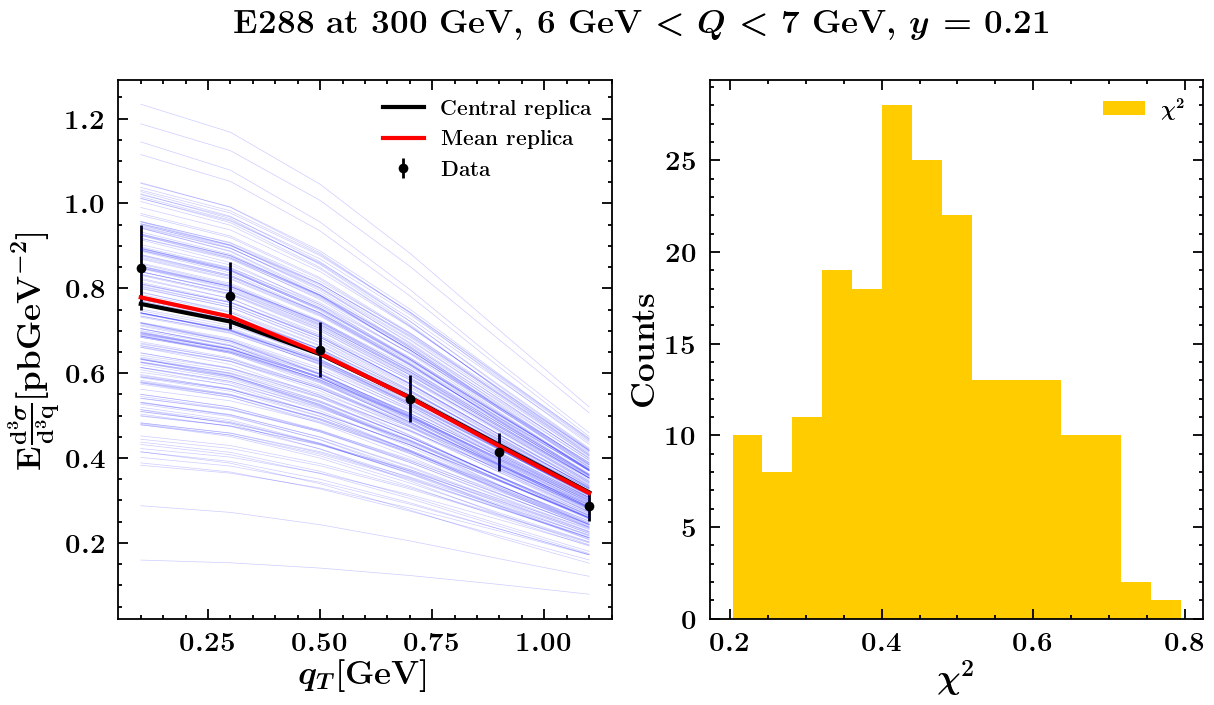
\includegraphics{pngplots/E288_300_Q_6_7.png}
\caption{E288\_300\_Q\_6\_7 data-theory comparison}
\end{figure}

\begin{figure}
\centering
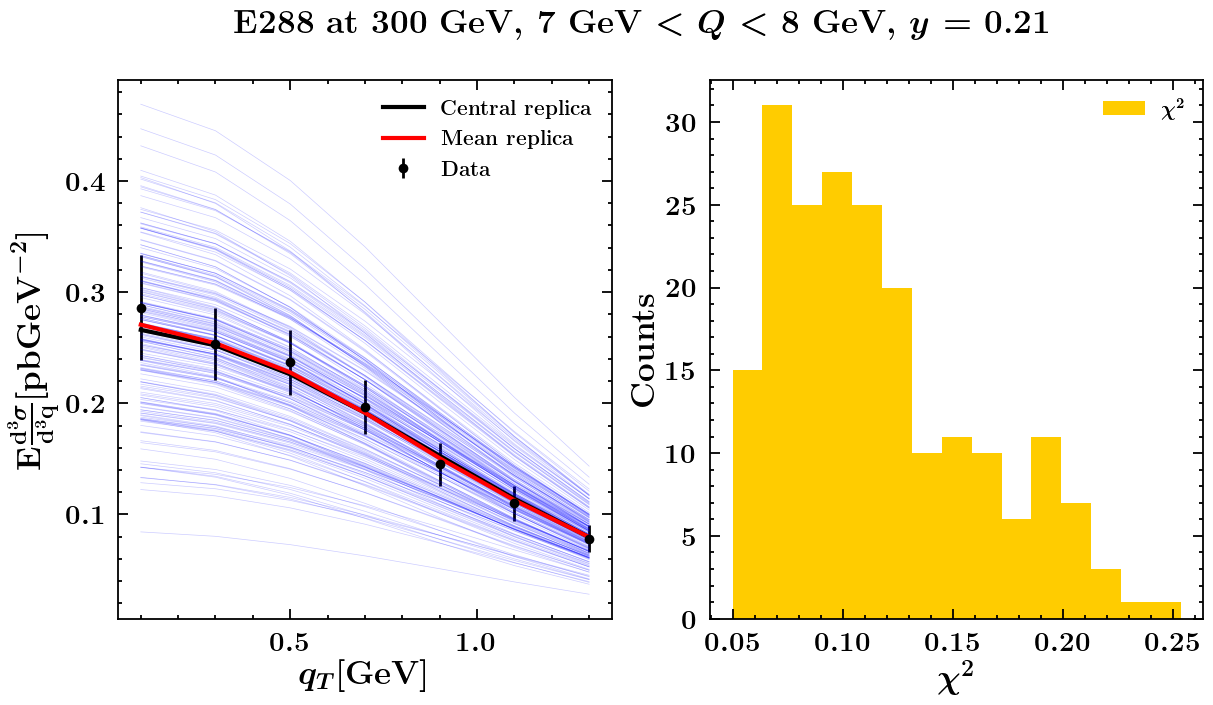
\includegraphics{pngplots/E288_300_Q_7_8.png}
\caption{E288\_300\_Q\_7\_8 data-theory comparison}
\end{figure}

\begin{figure}
\centering
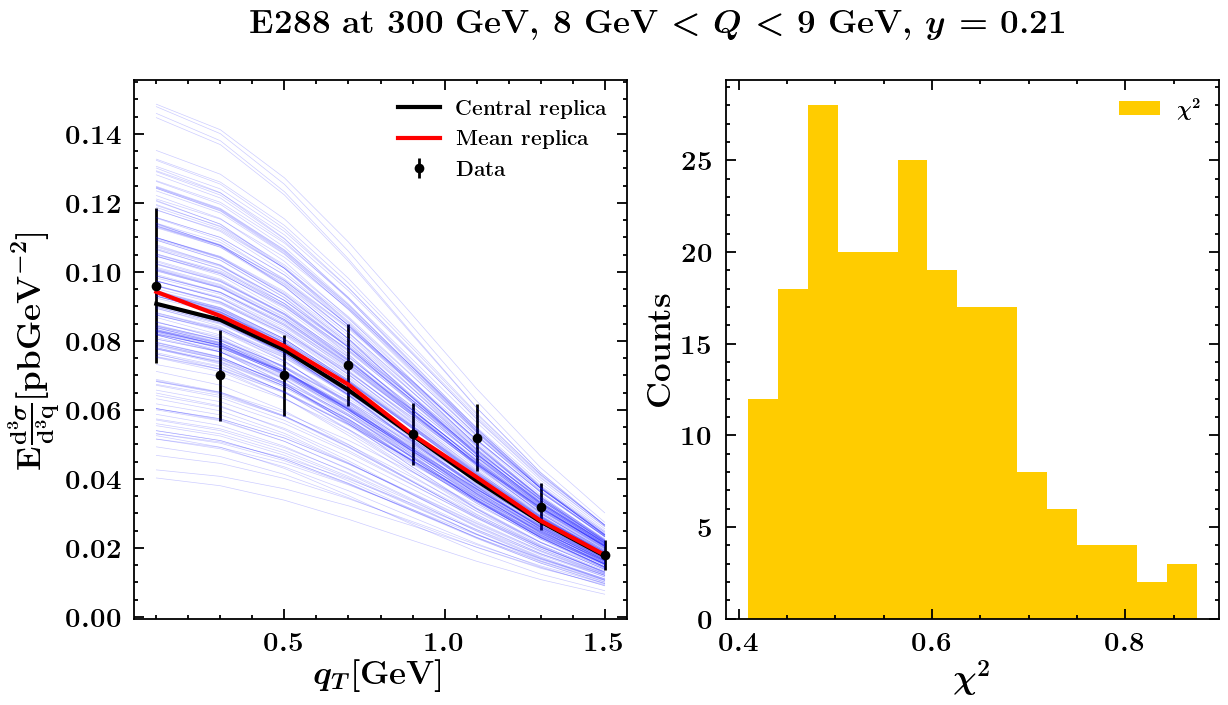
\includegraphics{pngplots/E288_300_Q_8_9.png}
\caption{E288\_300\_Q\_8\_9 data-theory comparison}
\end{figure}

\begin{figure}
\centering
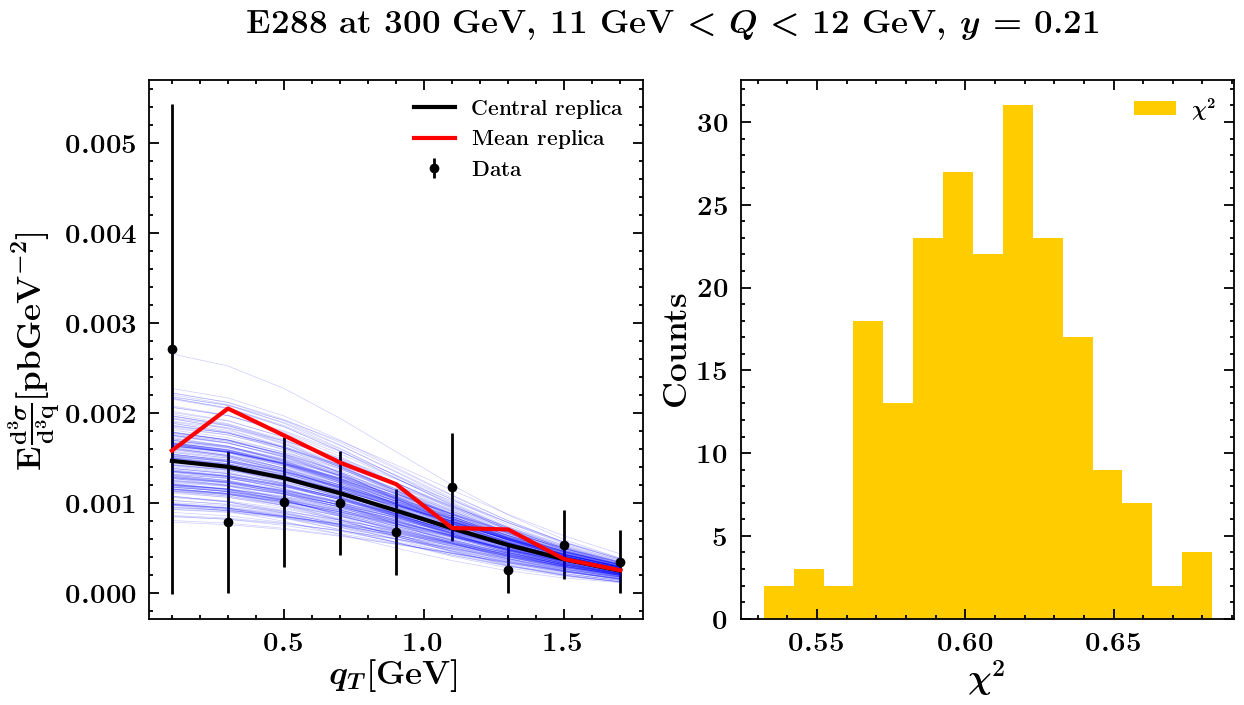
\includegraphics{pngplots/E288_300_Q_11_12.png}
\caption{E288\_300\_Q\_11\_12 data-theory comparison}
\end{figure}

\begin{figure}
\centering
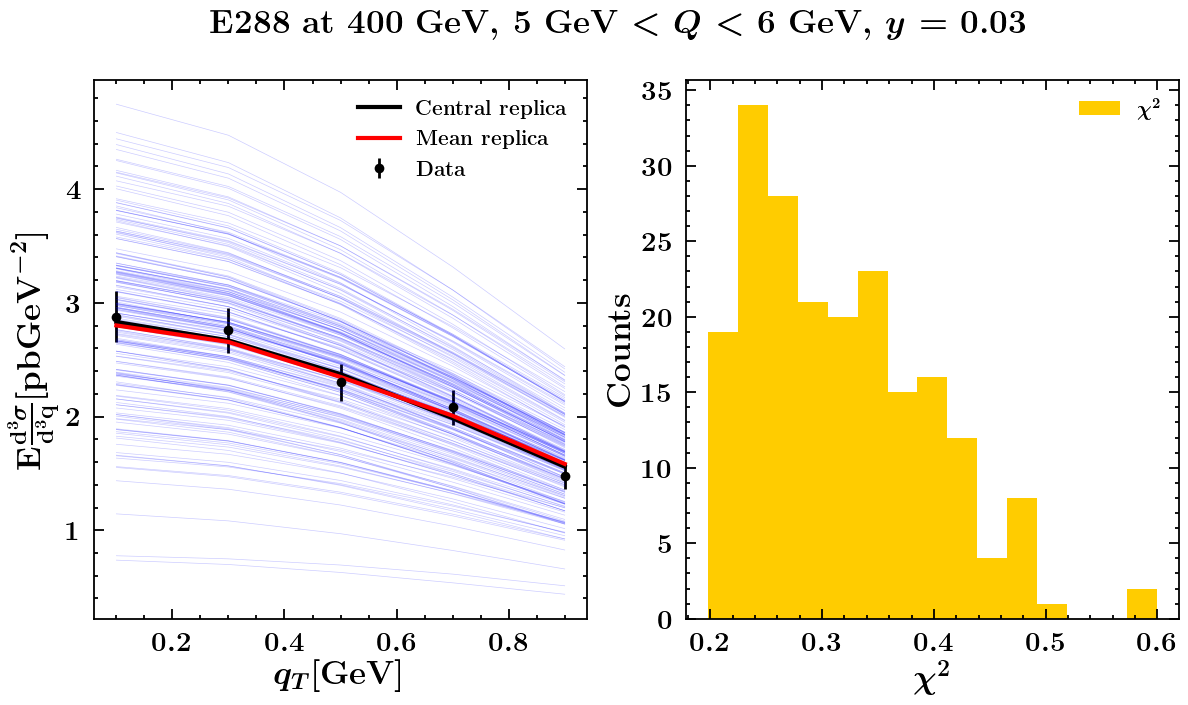
\includegraphics{pngplots/E288_400_Q_5_6.png}
\caption{E288\_400\_Q\_5\_6 data-theory comparison}
\end{figure}

\begin{figure}
\centering
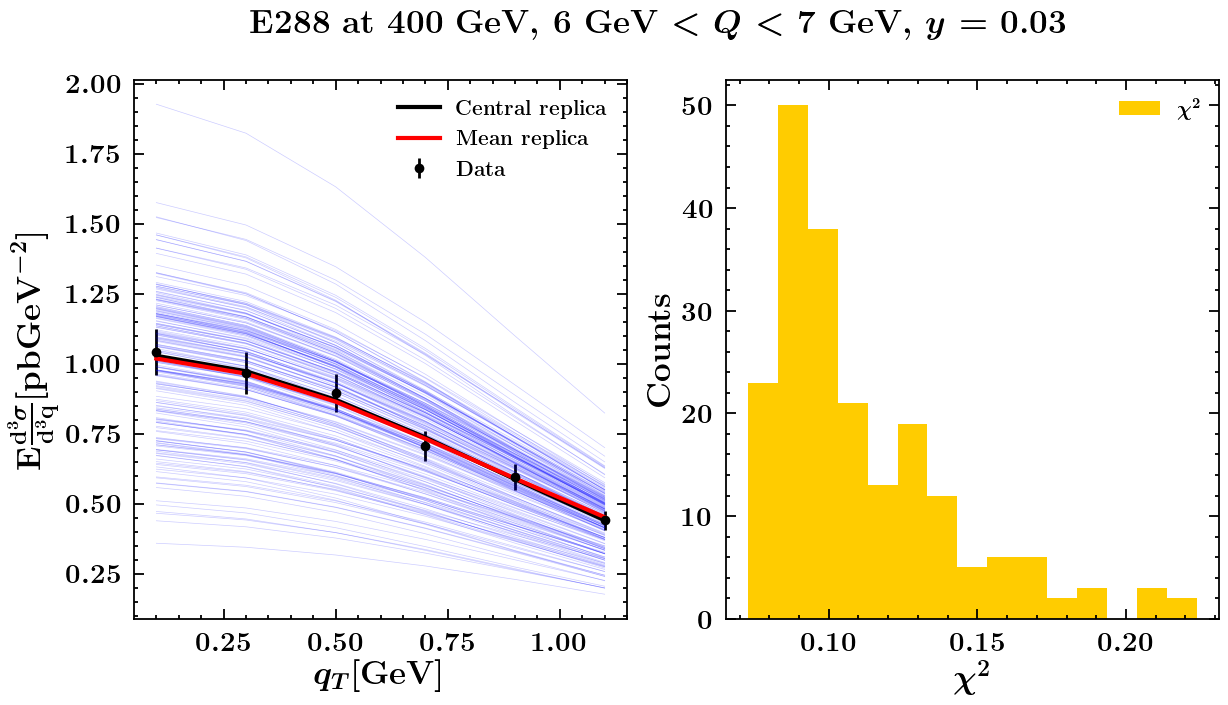
\includegraphics{pngplots/E288_400_Q_6_7.png}
\caption{E288\_400\_Q\_6\_7 data-theory comparison}
\end{figure}

\begin{figure}
\centering
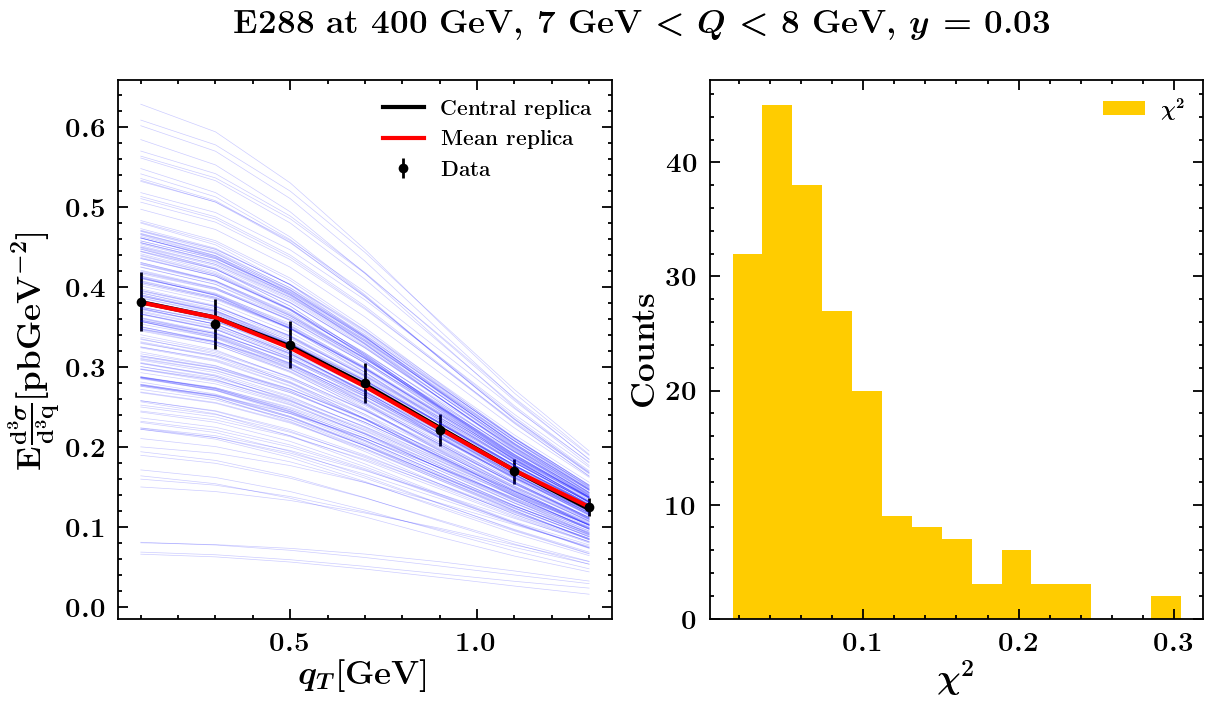
\includegraphics{pngplots/E288_400_Q_7_8.png}
\caption{E288\_400\_Q\_7\_8 data-theory comparison}
\end{figure}

\begin{figure}
\centering
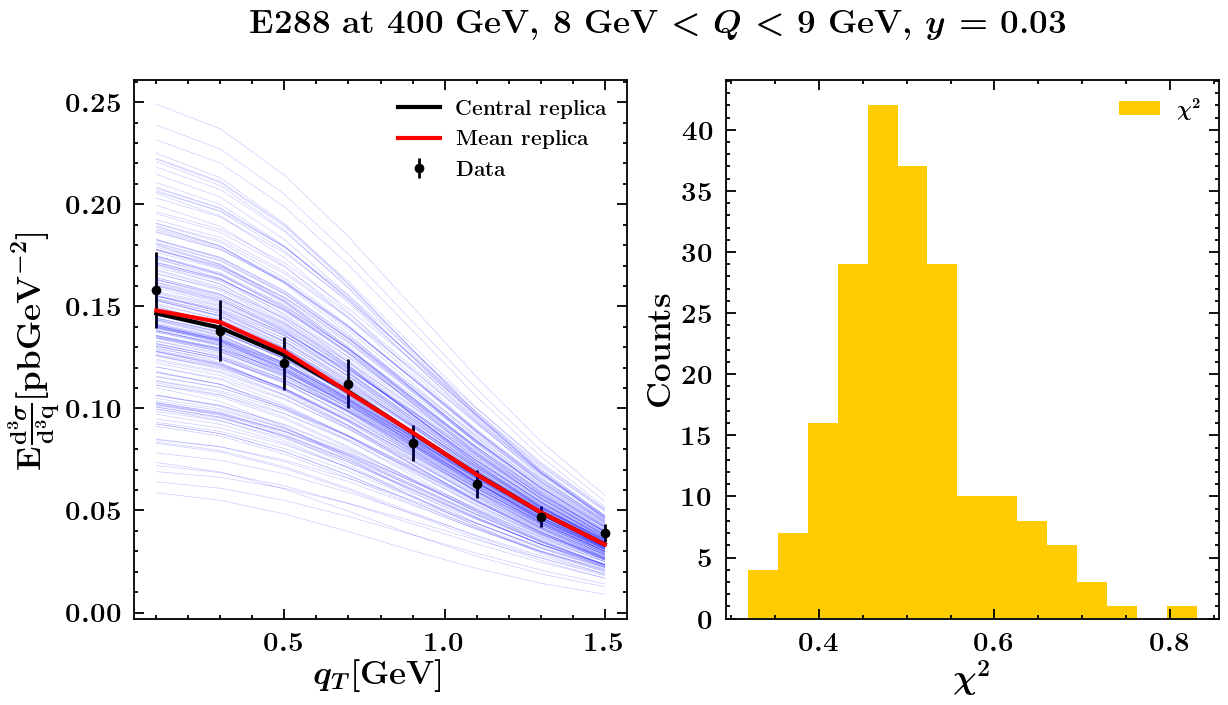
\includegraphics{pngplots/E288_400_Q_8_9.png}
\caption{E288\_400\_Q\_8\_9 data-theory comparison}
\end{figure}

\begin{figure}
\centering
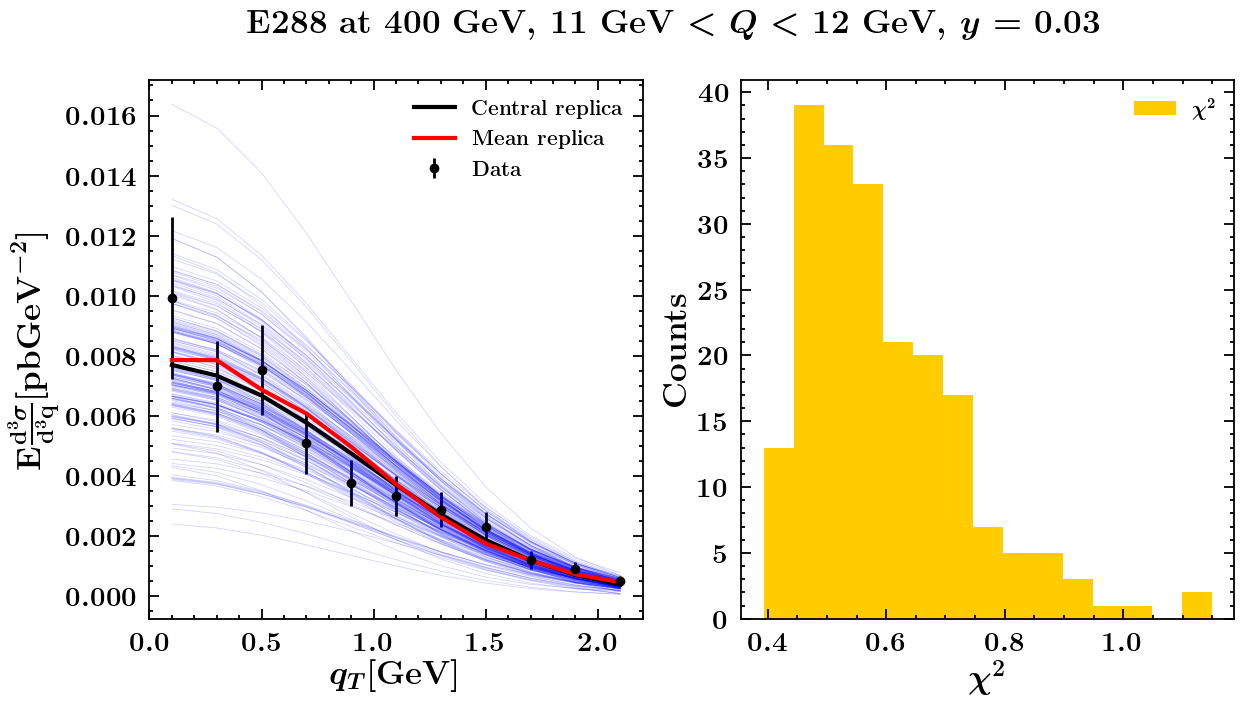
\includegraphics{pngplots/E288_400_Q_11_12.png}
\caption{E288\_400\_Q\_11\_12 data-theory comparison}
\end{figure}

\begin{figure}
\centering
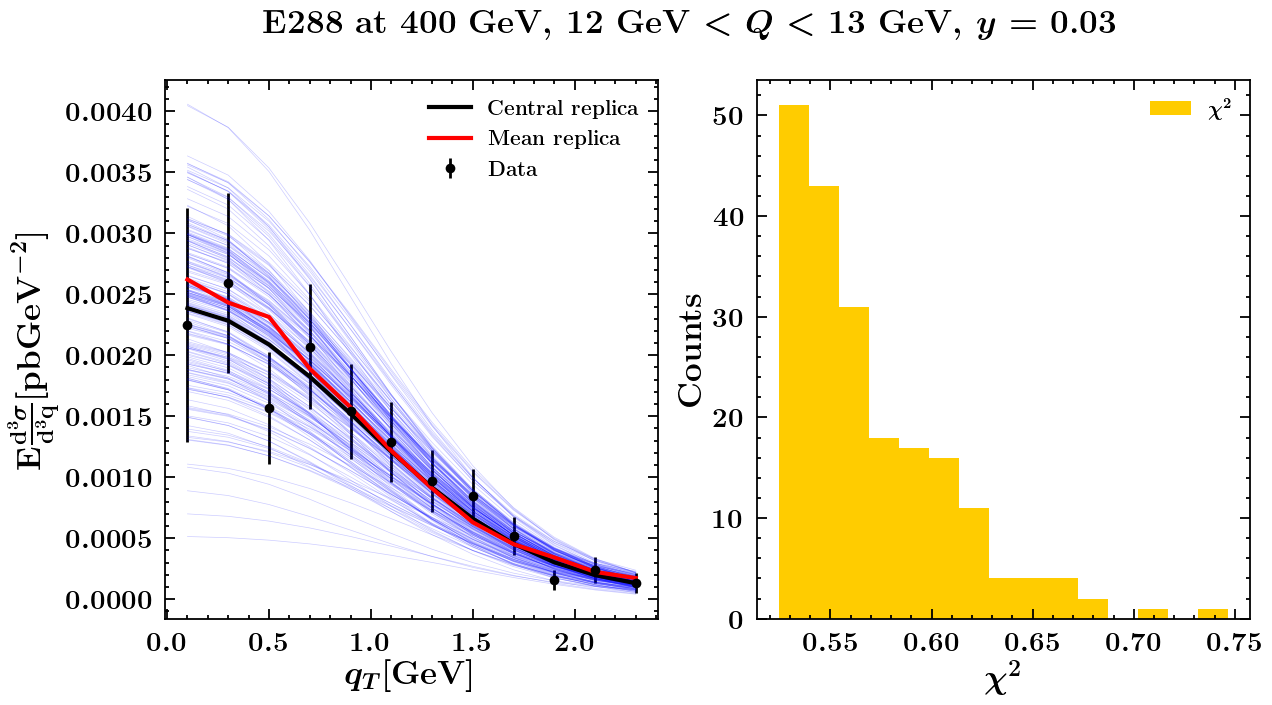
\includegraphics{pngplots/E288_400_Q_12_13.png}
\caption{E288\_400\_Q\_12\_13 data-theory comparison}
\end{figure}

\begin{figure}
\centering
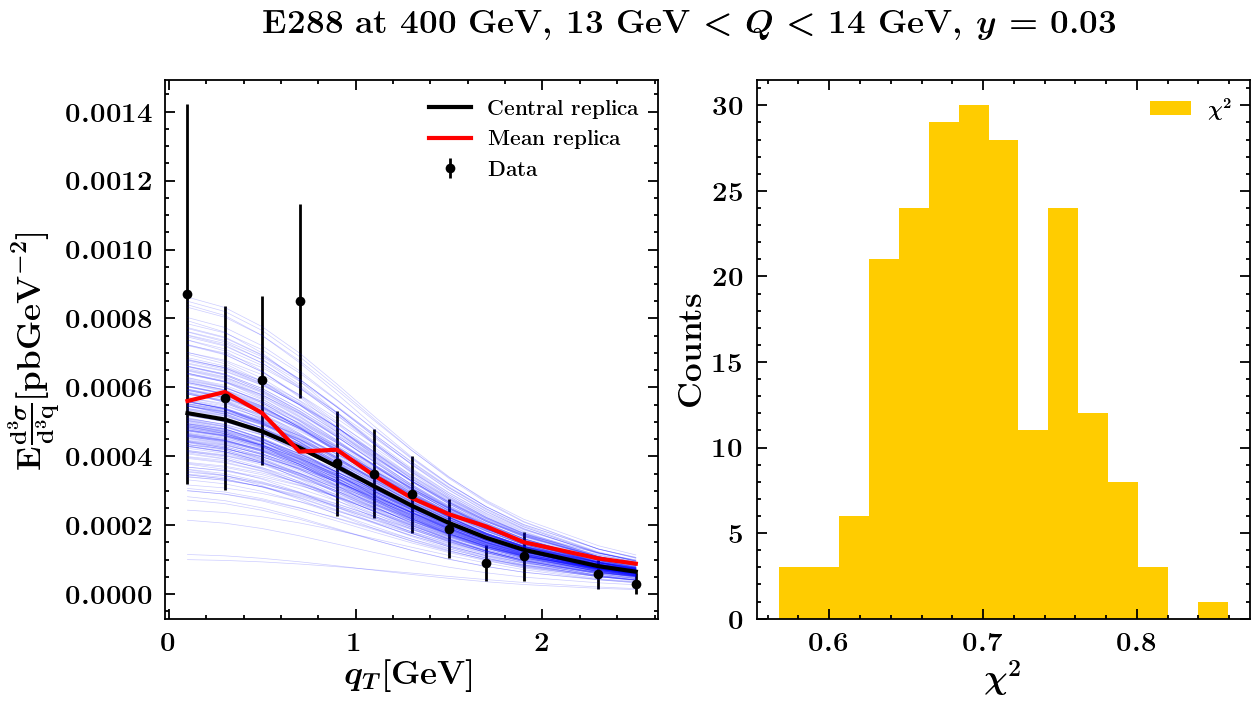
\includegraphics{pngplots/E288_400_Q_13_14.png}
\caption{E288\_400\_Q\_13\_14 data-theory comparison}
\end{figure}

\begin{figure}
\centering
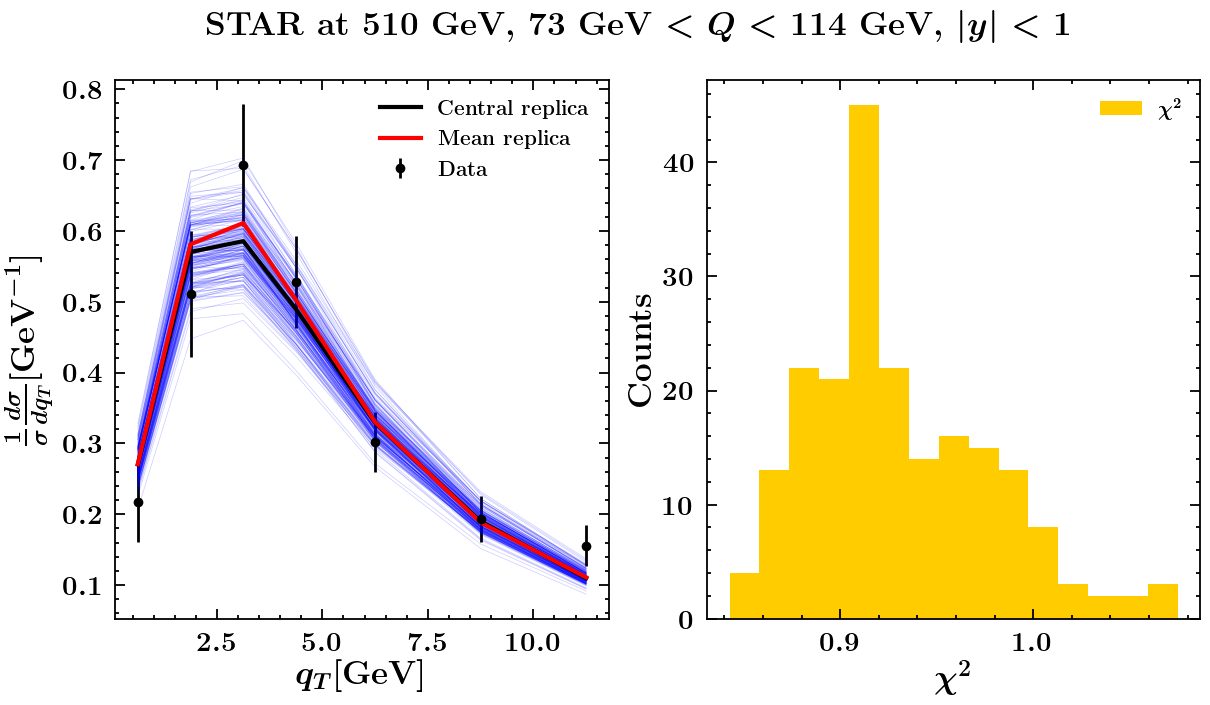
\includegraphics{pngplots/STAR_510.png}
\caption{STAR\_510 data-theory comparison}
\end{figure}

\begin{figure}
\centering
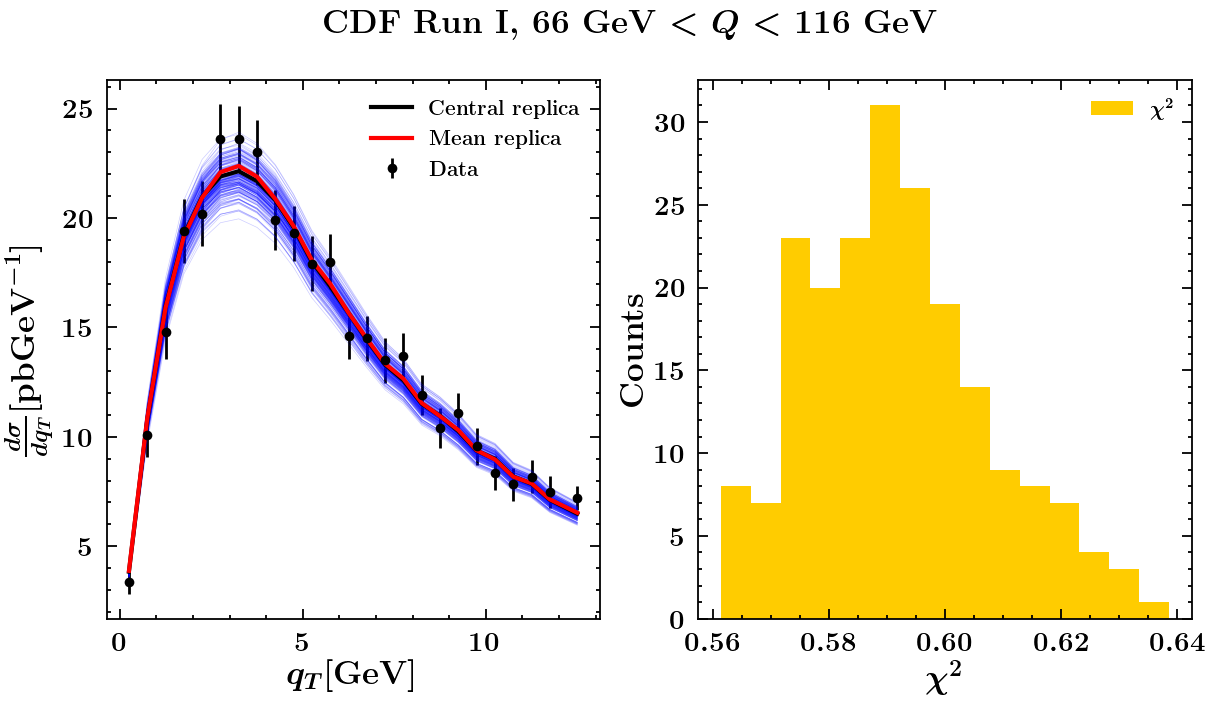
\includegraphics{pngplots/CDF_RunI.png}
\caption{CDF\_RunI data-theory comparison}
\end{figure}

\begin{figure}
\centering
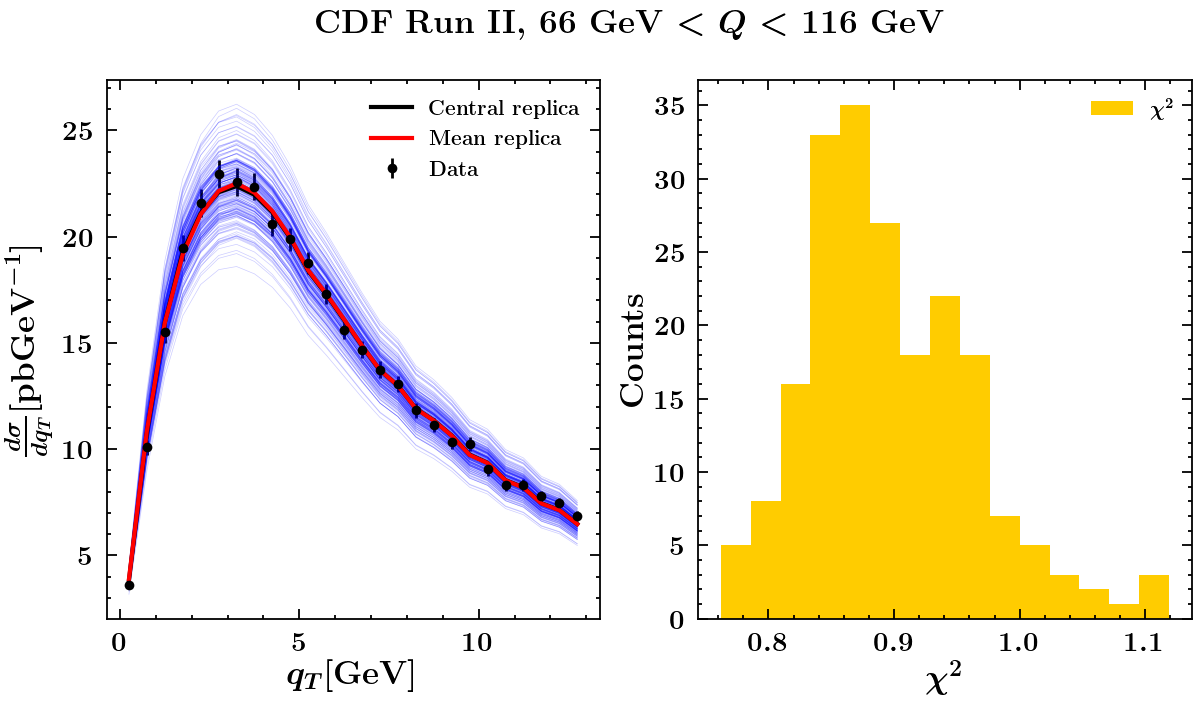
\includegraphics{pngplots/CDF_RunII.png}
\caption{CDF\_RunII data-theory comparison}
\end{figure}

\begin{figure}
\centering
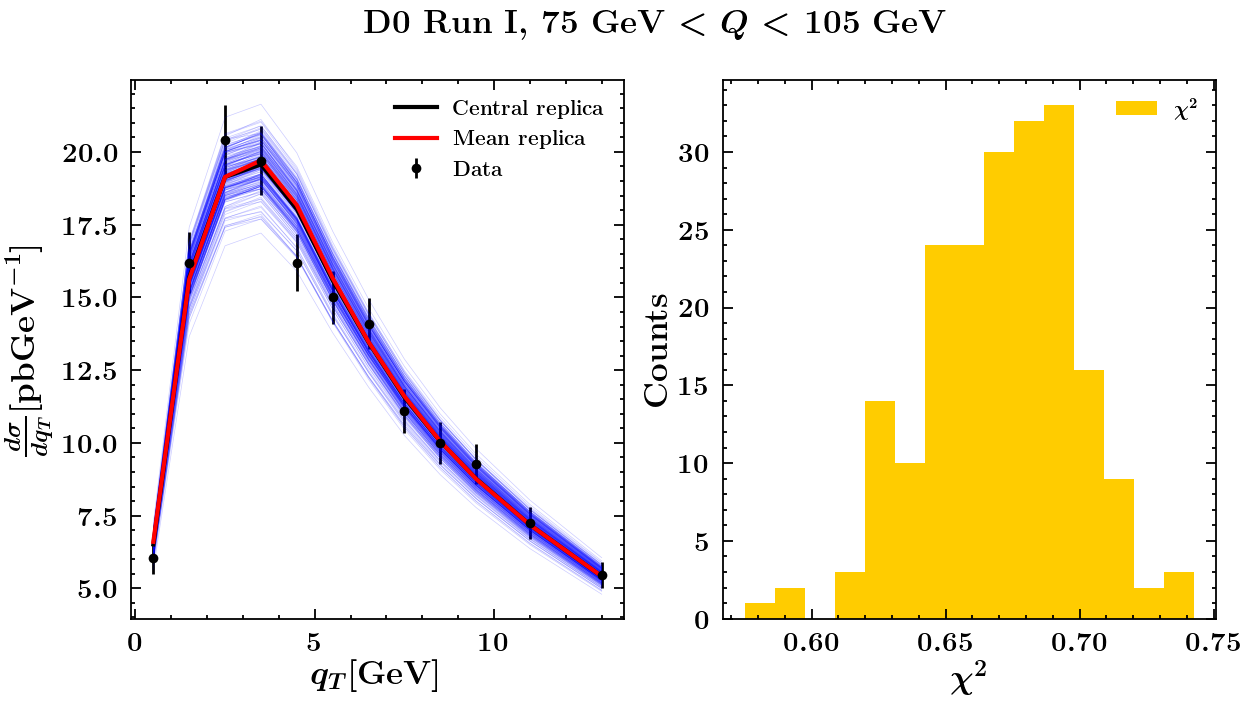
\includegraphics{pngplots/D0_RunI.png}
\caption{D0\_RunI data-theory comparison}
\end{figure}

\begin{figure}
\centering
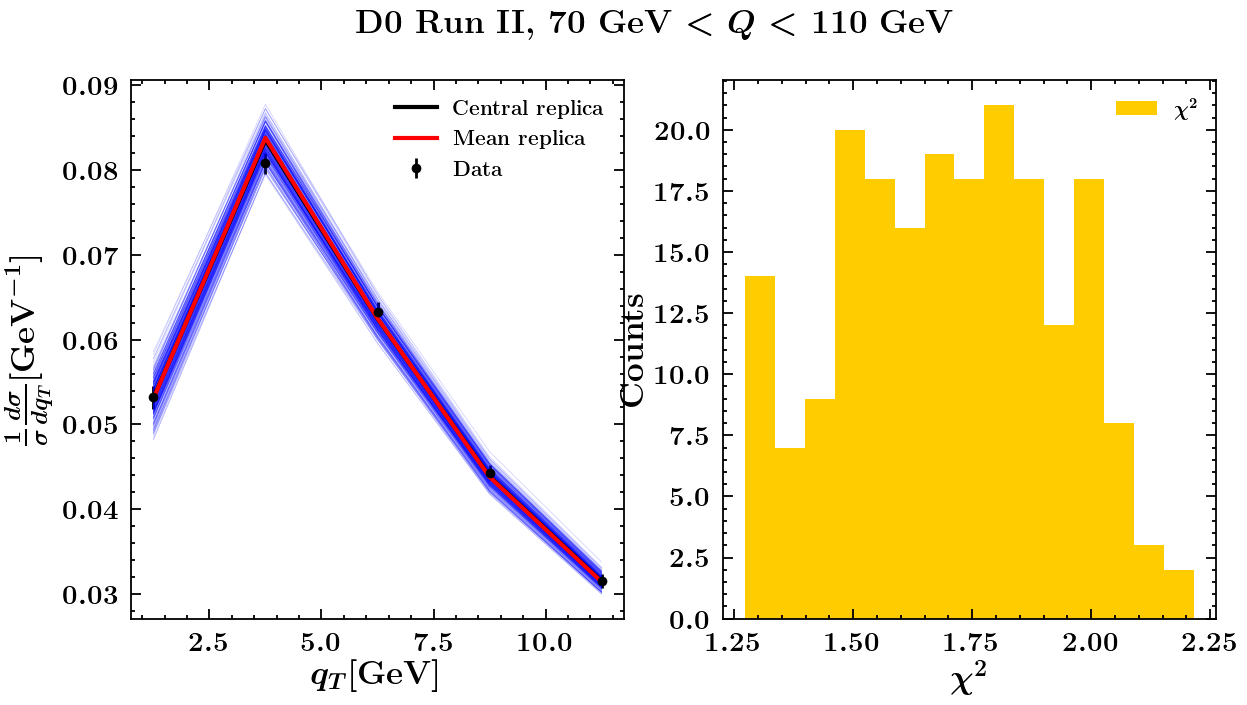
\includegraphics{pngplots/D0_RunII.png}
\caption{D0\_RunII data-theory comparison}
\end{figure}

\begin{figure}
\centering
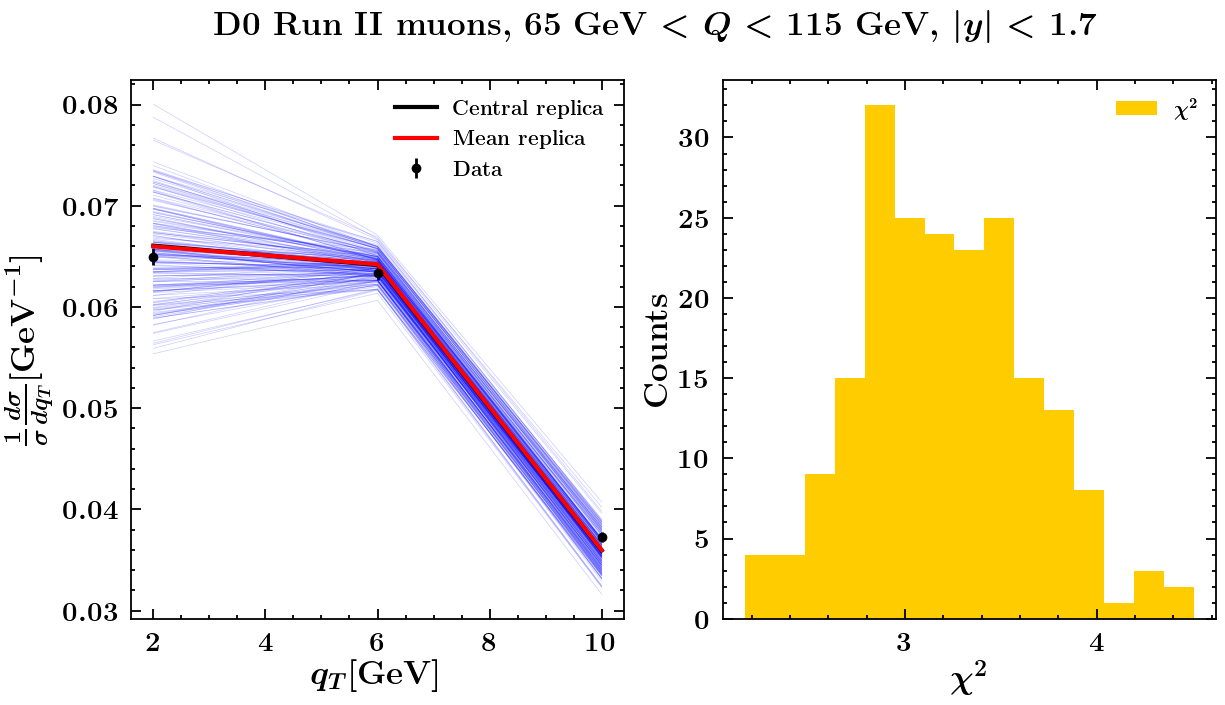
\includegraphics{pngplots/D0_RunIImu.png}
\caption{D0\_RunIImu data-theory comparison}
\end{figure}

\begin{figure}
\centering
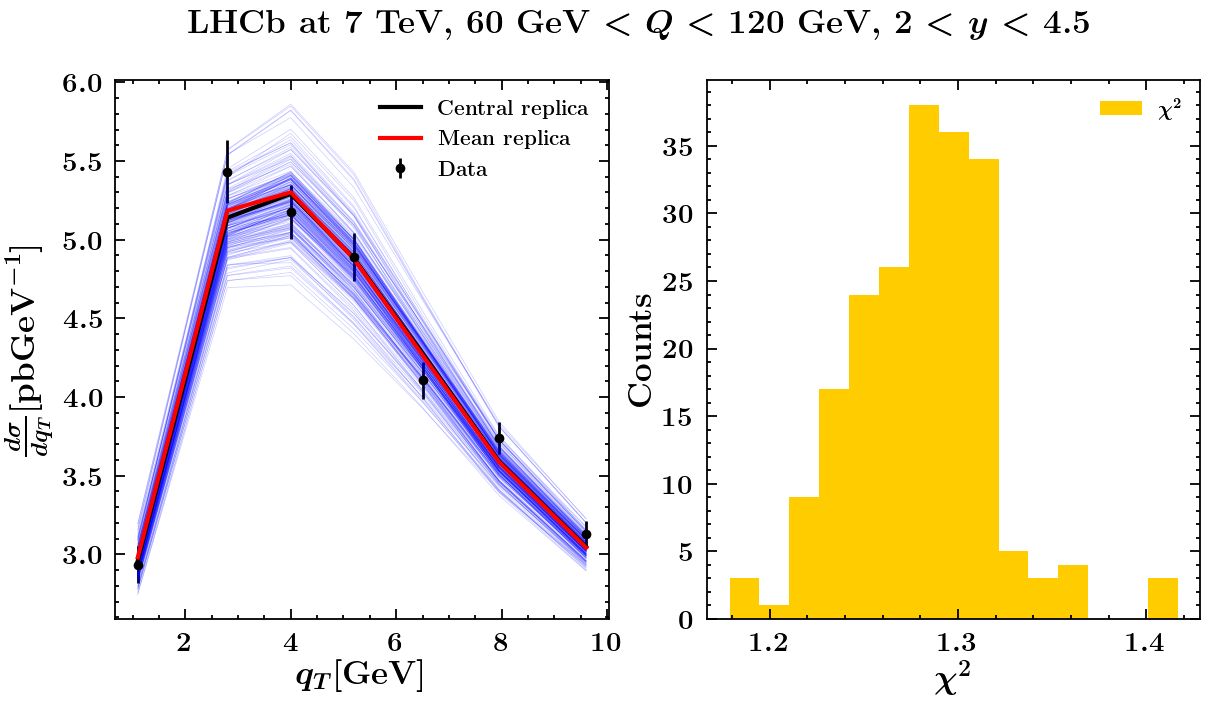
\includegraphics{pngplots/LHCb_7TeV.png}
\caption{LHCb\_7TeV data-theory comparison}
\end{figure}

\begin{figure}
\centering
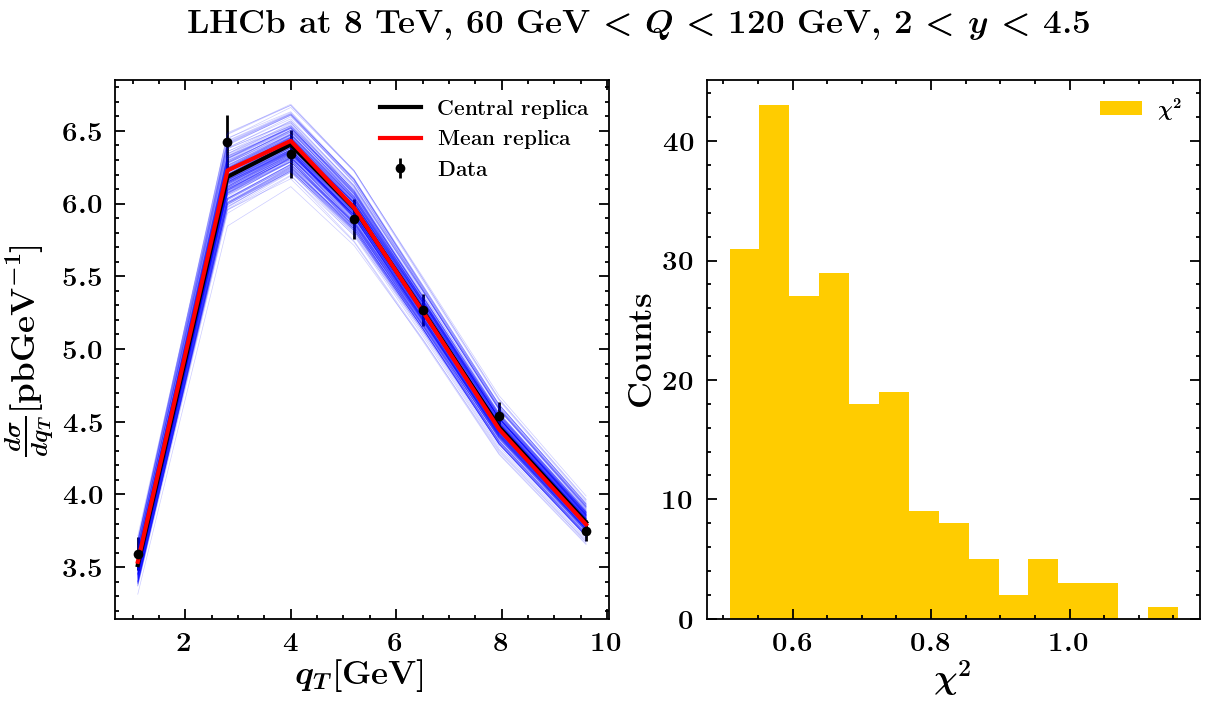
\includegraphics{pngplots/LHCb_8TeV.png}
\caption{LHCb\_8TeV data-theory comparison}
\end{figure}

\begin{figure}
\centering
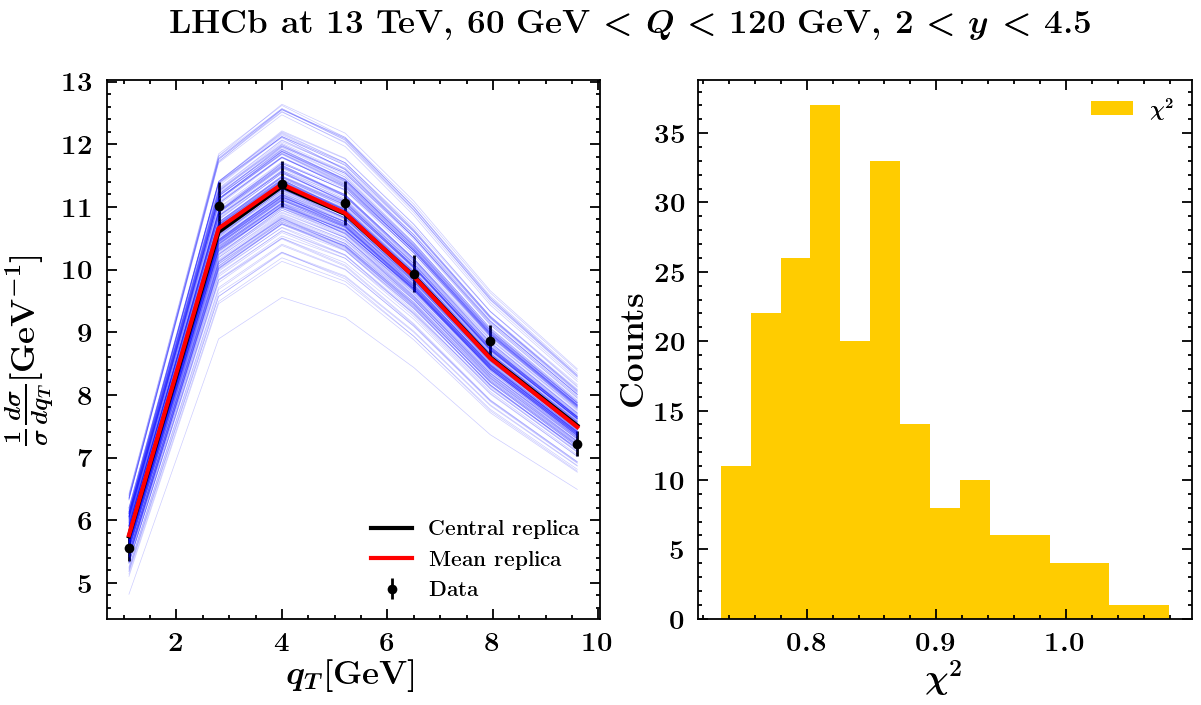
\includegraphics{pngplots/LHCb_13TeV.png}
\caption{LHCb\_13TeV data-theory comparison}
\end{figure}

\begin{figure}
\centering
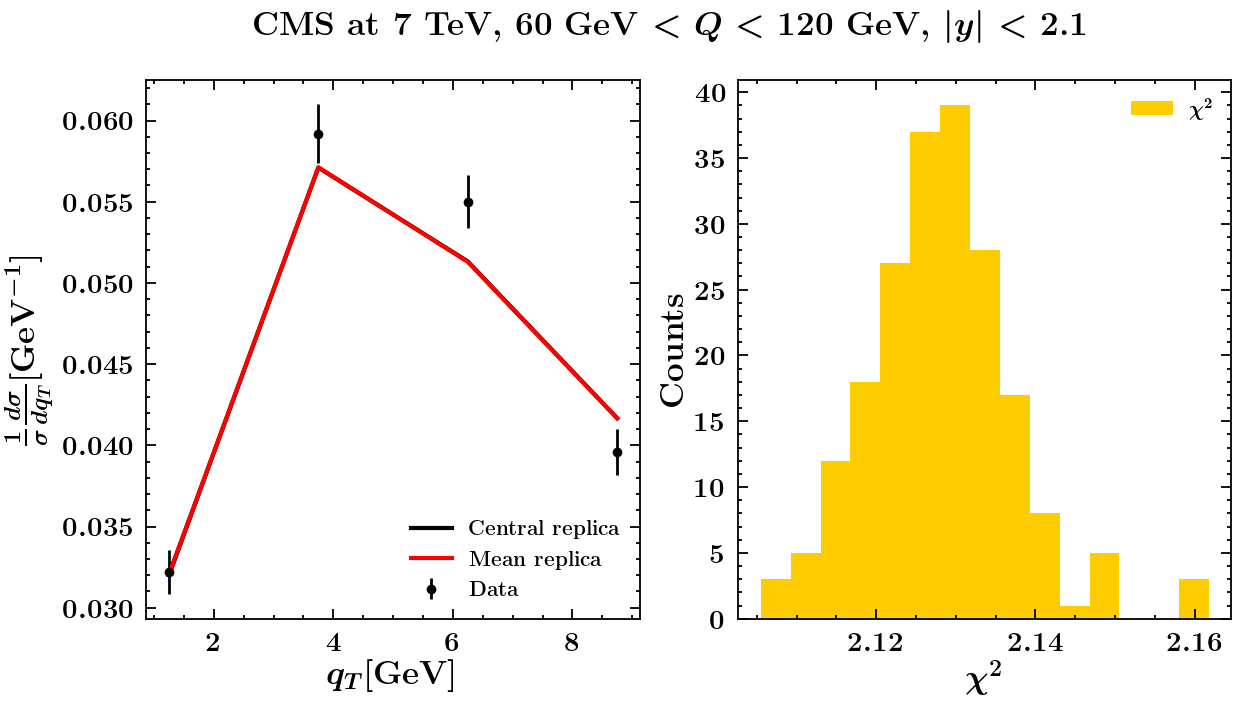
\includegraphics{pngplots/CMS_7TeV.png}
\caption{CMS\_7TeV data-theory comparison}
\end{figure}

\begin{figure}
\centering
\includegraphics{pngplots/CMS_8TeV.png}
\caption{CMS\_8TeV data-theory comparison}
\end{figure}

\begin{figure}
\centering
\includegraphics{pngplots/ATLAS_7TeV_y_0_1.png}
\caption{ATLAS\_7TeV\_y\_0\_1 data-theory comparison}
\end{figure}

\begin{figure}
\centering
\includegraphics{pngplots/ATLAS_7TeV_y_1_2.png}
\caption{ATLAS\_7TeV\_y\_1\_2 data-theory comparison}
\end{figure}

\begin{figure}
\centering
\includegraphics{pngplots/ATLAS_7TeV_y_2_2.4.png}
\caption{ATLAS\_7TeV\_y\_2\_2.4 data-theory comparison}
\end{figure}

\begin{figure}
\centering
\includegraphics{pngplots/ATLAS_8TeV_y_0_0.4.png}
\caption{ATLAS\_8TeV\_y\_0\_0.4 data-theory comparison}
\end{figure}

\begin{figure}
\centering
\includegraphics{pngplots/ATLAS_8TeV_y_0.4_0.8.png}
\caption{ATLAS\_8TeV\_y\_0.4\_0.8 data-theory comparison}
\end{figure}

\begin{figure}
\centering
\includegraphics{pngplots/ATLAS_8TeV_y_0.8_1.2.png}
\caption{ATLAS\_8TeV\_y\_0.8\_1.2 data-theory comparison}
\end{figure}

\begin{figure}
\centering
\includegraphics{pngplots/ATLAS_8TeV_y_1.2_1.6.png}
\caption{ATLAS\_8TeV\_y\_1.2\_1.6 data-theory comparison}
\end{figure}

\begin{figure}
\centering
\includegraphics{pngplots/ATLAS_8TeV_y_1.6_2.png}
\caption{ATLAS\_8TeV\_y\_1.6\_2 data-theory comparison}
\end{figure}

\begin{figure}
\centering
\includegraphics{pngplots/ATLAS_8TeV_y_2_2.4.png}
\caption{ATLAS\_8TeV\_y\_2\_2.4 data-theory comparison}
\end{figure}

\begin{figure}
\centering
\includegraphics{pngplots/ATLAS_8TeV_Q_46_66.png}
\caption{ATLAS\_8TeV\_Q\_46\_66 data-theory comparison}
\end{figure}

\begin{figure}
\centering
\includegraphics{pngplots/ATLAS_8TeV_Q_116_150.png}
\caption{ATLAS\_8TeV\_Q\_116\_150 data-theory comparison}
\end{figure}

\end{document}
